\documentclass[twoside,11pt]{starlink}

% -----------------------------------------------------------------------------
% ? Document identification
\stardoccategory    {Starlink User Note}
\stardocinitials    {SUN}
\stardocsource      {sun\stardocnumber}
\stardocnumber      {161.2}
\stardocauthors     {D C Parsons, D S Berry, W Gong, H J Walker}
\stardocdate        {10 November 1994}
\stardoctitle     {IRAS90\\[2ex]
                                Introductory/User Guide to\\[2ex]
                                Calibrated Reconstructed Detector\\[2ex]
                                Data Analysis}
\stardocabstract  {
IRAS90 is a suite of programs for processing IRAS data. It takes advantage
of Starlink's ADAM environment, which provides multi-platform availability
of both data and the programs to process it, and the user friendly interface of
the parameter entry system.
}
% ? End of document identification

% -----------------------------------------------------------------------------

% ? Document-specific \providecommand or \newenvironment commands.
% ? End of document-specific commands
% -----------------------------------------------------------------------------
%  Title Page.
%  ===========
\begin{document}
\scfrontmatter

\section{Introduction
\xlabel{introduction}\label{m:intro}}

IRAS90 is a new suite of programs for processing IRAS data. It takes advantage
of the ADAM environment on Starlink, which provides multi-platform availability
of both data and the programs to process it, and the user friendly interface of
the parameter entry system.

A brief introduction to all the data products prepared from the IRAS mission
is given in the IRAS Data Products Primer
\xref{SUN/82}{sun82}{}. IRAS90 applications cover
processing of the CRDD data (described below), IRAS image data of various types,
and provide facilities to augment image display and processing routines with
information based on position in the standard Astronomical coordinate systems.
It does not process either IRAS catalogues or IRAS Low Resolution Spectra.

There are at present TWO documents describing the IRAS90 applications. This is
the more elementary and is aimed specifically at the user of IRAS CRDD. Full
details of all the options in the IRAS90 applications can be found in
\xref{SUN/163}{sun163}{}
`IRAS90 - Survey and PO Data Analysis Package - Reference Guide'.


This document aims to answer the following questions :-
\begin{itemize}

\item It gives background information for people new to CRDD processing in
Sections \ref{m:crdd} and \ref{m:stagcrdd}.

\item It gives comparison information for users of the previous processing
system, in Sections \ref{m:newfac} and \ref{m:oldnew}.

\item It describes the information needed, and the instructions that must be
given, to carry out the process of preparing and examining an image from CRDD,
or detecting a point source.

Applications can be run in default mode, which adopts the most usual form of
processing, or in a wide variety of alternatives specified by entering parameter
values on the command line which requests the application. In this document a
series of walkthroughs showing the command lines and output from each
application running in default mode are given, together with details of the
information the user needs to run the application. These are given in
Sections \ref{m:extract} to \ref{m:coadd}.

This document aims to give details of a straightforward, but complete processing
run. Therefore it includes details of some KAPPA applications where these are
combined with IRAS90 astrometric applications for examining images. However it
does not treat IRAS90 applications which are used for tasks other than the
straightforward processing run.

This document aims not to make any prior assumptions about the users knowledge.
Therefore a user familiar with the ADAM environment need only consult Section
\ref{m:useadam} to obtain information on how to start IRAS90. A user familiar
with KAPPA may only wish to read section \ref{m:kappa1} to find out how KAPPA
applications mesh with IRAS90 astrometric applications. However most users will
need to read Section \ref{m:promult} to find out how to specify processing of
multiple files.

\item The user needs to have a brief overview of the way in which his data has
been processed in order to determine whether it has been processed in a way he
feels to be satisfactory. This is described in the `process' subsections of
Sections \ref{m:destback} and \ref{m:mapcrdd}. If he does not feel that
the processing is suitable then he can consult
\xref{SUN/163}{sun163}{} to read further details
of the alternatives available to him.

\item This document gives a complete list of all IRAS90 applications, classified
by their function in Section \ref{m:otheriras90}.

Full details of all IRAS90 applications are given in
\xref{SUN/163}{sun163}{}. This includes
details of applications not in the straightforward processing run, and
therefore omitted from this document. The details of individual application
describe all the parameters in alphabetical order which may be a little
confusing at first. It is therefore suggested that a novice user becomes
familiar with the default option walkthroughs given in this document, before
embarking on the more detailed documentation.
\end{itemize}

The user should note that all IRAS90 and KAPPA applications use Starlink
standard .SDF format files, which are portable between Vax and Unix systems.
However the program I\_COADD which is used to detect point sources, has not
yet been replaced and uses the old .BDF format files. These can only be
processed on a Vax. Information about obtaining the correct data is contained
in Section \ref{m:exinfo}, and information about translation from .BDF to .SDF
formats is found in Appendix \ref{a:ndfout}.

The Appendices provide additional information as follows
\begin{itemize}
\item Appendix \ref{a:a} contains the graphical output from the KAPPA
walkthrough and comparison between IRAS90 and the previous IRAS processing
suite.
\item Appendix \ref{a:fulldbm} contains a walkthrough of the non defaulted
destriping, background removal and making an image applications.
\item Appendix \ref{a:exkappa} contains extended examples of using IRAS90
astrometric applications with KAPPA.
\item Appendix \ref{a:quality} contains details of quality handling.
\item Appendix \ref{a:ndfout} contains information about translation from
.BDF to .SDF formats.
\item Appendix \ref{a:docs} gives references to further documentation on IRAS90,
and other more general information.
\end{itemize}

For ease of readability, I have referred to the user throughout this document
as he, rather than he or she, and I hope that those amongst its readership
who, like me, are female will excuse me.

\section{Calibrated Reconstructed Detector Data
\xlabel{calibrated_reconstructed_detector_data}\label{m:crdd}}

\subsection{Why process CRDD data ?}
The whole sky survey data from the IRAS mission have been processed in several
ways to give for example the Point Source Catalogue (IRPS in the STADAT list)
and the sky flux plates. In general, the processing used to derive these
products was somewhat conservative in order to achieve a high reliability for
the PSC sources and a uniform resolution among the bands for sky flux plates.
However, if a lower reliability is accepted fainter sources can be extracted
from the data, and a relaxation of the resolution uniformity requirement allows
more spatial information to be preserved in the construction of images.
Complete details of the reliability, completeness, and resolution of the
processed data can be found in the `IRAS Catalogues and Atlases Explanatory
Supplement'.

The Calibrated Reconstructed Detector Data (CRDD) has been made available so
that astronomers can process it themselves to obtain data of whatever standard
they feel is acceptable. The Explanatory Supplement gives the necessary details
of the sampling procedure and the inherent reliability considerations.

However, processing CRDD is not a task to be undertaken lightly. The data is
voluminous and processing it takes a lot of both the user's and the computer's
time. It is always worthwhile looking at the processed data available to see
whether it is suitable before embarking on CRDD processing.

\subsection{What is CRDD data ?}

The following provides only a brief introduction to CRDD data, more detailed
notes on how the raw data was collected and the processing that was carried out
on it to prepare the  calibrated reconstructed detector data can be found in
the Explanatory Supplement. Details of a later recalibrated version of
essentially the same data (PASS3 CRDD) will be referenced in the online help
associated with the IRAS90 suite when it becomes available.

The CRDD data comprises the minimally processed data for the IRAS whole sky
survey.

The IRAS mission gave strips of data, called survey observations, as the
detectors scanned the sky from South ecliptic pole to North ecliptic pole
approximately (or vice versa). Observations were carried out in such a way that
successive ones half overlapped. This would enable two sets of data covering
the same section of sky and close in time to be compared so that the most
obvious inconsistencies could be removed. This group of observations is termed
an HCON (for Hours Confirmed). Similar sets of observations would be made
about 2 weeks later, and 6 months later for 72\% of the sky. In the survey any
particular position in the sky was covered up to 6 times.

The data obtained in the survey was subsequently calibrated using the internal
calibrator and NGC6543 (after removal of detector noise), as described in the
Explanatory Supplement section VI (A4 and B).

The data as the user will extract it, or receive it, will be a set of `scan'
files.
\begin{itemize}
\item A scan is length of data from a single observation, started and ended as
it crosses into and out of the region of interest area the user specified
around his source. As the user specifies this area in coordinates which
correspond to the geometry of the observations, the combined scans from any
HCON will form an approximate parallelogram at an angle to the more usual
equatorial coordinate system. Different HCONs may scan in different directions.
\item The scan file contains data for one waveband only. It consists of the
samples of data from each detector which operated in the waveband specified,
the samples being all those taken in the scan length.
\item The scan also contains the positional information that identifies the
track of the scan across the sky.
\end{itemize}

The CRDD data archive is held as files called plates. Each plate contains all
the sections of observations which cross a region of sky corresponding to the
region covered by a Palomar Sky Plate. Although the plates overlap by about a
degree at each edge, some of the big regions of interest will fall over the
boundaries of a plate. Usually only the data from the plate containing the
source position will be extracted. But if this is insufficient, data can be
supplied from two plates. However normal processing may lead to different
background estimates being subtracted from each half.

One further term that should be explained is that of a SOP. The IRAS
observations were scheduled in roughly 12 hour periods called Satellite
Operations Plans, SOPs. A SOP consisted of a number of observations which
contributed to the whole sky survey, together with Pointed Observations (POs)
giving greater resolution for scanning of particular objects. (The latter may be
referred to as Additional Observations in other documentation). As observations
for a given HCON were collected either on different parts of the same SOP, or
on consecutive SOPs, examination of the SOP number of a scan is a good indicator
of to which HCON it belongs.

If you are using CRDD data to estimate whether there is a source at a given
position you should bear in mind that each point on the sky is crossed
typically by 12 detectors in each band. Individual traces may not show any
obvious signal but the expected improvement arising from COADDing the
individual detector data may give a significant signal.

\section{Stages in Calibrated Reconstructed Detector Data processing
\xlabel{stages_in_crud_data_processing}\label{m:stagcrdd}}

There are two types of processing that the user would normally want to carry
out on CRDD data, to prepare an image of a source region, and to find out
whether there is a significant source at a particular position and measure its
flux.

The first stage in either case is to extract the data for the region of
interest from the data archive tapes.

The processing of CRDD data to make images then consists of
\begin{itemize}
\item Forming an image from the data as follows
\begin{itemize}
\item Each detector has its own differences in calibration, which means that
two detectors each looking at the same piece of sky would give a different
background level. By destriping the user can adjust detector levels within a
scan to reduce this effect substantially. This process is carried out by
DESTCRDD.
\item After destriping there  still remains a background flux level which, when
scans are combined together, will give a striped effect. The user may remove
this either as a constant value, or as a value with linear gradient along the
scan, by using the BACKCRDD application. We hope to be able to provide more
sophisticated background removal algorithms, such as ones based on zodiacal
light, in future releases of IRAS90.
\item Finally the individual detector samples are joined together to form an
image taking into account the fact that detectors from adjacent scans half
overlap on the sky, and the resulting image is rebinned onto a new matrix of
pixels whose orientation can be specified by the user. This is usually parallel
to the users chosen astronomical coordinate system. This is done by the MAPCRDD
application.
\item The user can also examine pictorial representations of the detector data
stream before processing, or after the destriping or background removal stages.
He can use this to determine which type of background he should remove, or to
determine parameters for omitting point sources, as well as any checking of
the final result. The application which provides this is called TRACECRDD.
\end{itemize}
\item Examining the image
\begin{itemize}
\item To examine an IRAS image a user  should now use KAPPA. The KAPPA suite
offers a wide variety of applications to display and manipulate images.
Facilities for obtaining and displaying positional information in standard
astronomical coordinate systems, can now be used with KAPPA. This has been
developed by the IRAS90 team  and can be used with any image carrying IRAS-type
astrometry information.
Thus, using KAPPA, a user can prepare a grey scale image, or contour map, or
both combined, with appropriate grids, keys and annotations, and obtain printed
copies of them. He can also obtain flux values for positions determined in
various  ways including those at given sky coordinate values.
\end{itemize}
\end{itemize}

The processing of CRDD data to determine whether there is a significant source
at a point, and determine its flux consists of
\begin{itemize}
\item Combining detector data using the COADD program, which combines detectors
from several scans as they cross the source position. This gives a better
signal to noise and enables faint sources to be detected and more accurate flux
determinations to be made.
However, the IRAS90 COADD program is currently being written and therefore is
not in the first release. Users wishing to COADD sources will have to use the
old IRAS I\_COADD program and the old data format. If they also want to use
TRACECRDD they will need both formats of data or be willing to use NDFOUT from
EDRSX to change old .BDF data format files to new .SDF data format files.
Details of how to use NDFOUT are given in Appendix \ref{a:ndfout}.
\item Using TRACECRDD to look at a pictorial representation of the detector
data. This is particularly useful if he is unsure of whether his source is a
point source or extended, as the COADD program assumes a point source.
TRACECRDD provides point source profiles.
However the user should be aware that because he is examining single detector
traces each may look as if there is only noisy background at the source point,
where the COADD program which adds detectors may reveal sufficient signal.
\end{itemize}
\section{New facilities provided by the IRAS90 suite
\xlabel{new_facilities_provided_by_iras90}\label{m:newfac}}

IRAS90 provides the following improvements over the old I\_ IRAS suite
\begin{itemize}
\item The programs are now available through the Starlink ADAM environment.
Which
means that users can work on either a Vax machine under DCL, or ICL, or a Unix
machine interchangeably. The user meets the same interface for each application,
and data can be used under either operating system without translation.
\item The ADAM parameter and help systems provide a more friendly and uniform
user interface. The inexperienced user finds it easier to operate the
applications as the more unusual options are hidden. While these options can
be called upon by command line specifications by the more experienced.
\item The IRAS90 programs are more flexible and more controllable than the
corresponding I\_ routines.
\item Users are allowed to specify source positions in several standard
Astronomical coordinate systems.
\item The tedium of processing files through the old IRAS applications has
been relieved by the ability to specify that multiple files should be processed
with one command for certain applications.
\item New facilities for examining detector data, assigning qualities to
detector samples or image pixels, and processing according to those qualities,
have been incorporated in the suite.
\item The IRAS user can now have easy access to the flexible image processing
capabilities of KAPPA. KAPPA facilities can now be interleaved with IRAS90
applications which allow the user to draw grids, mark, annotate and
identify positions in the standard Astronomical coordinate systems, as was
provided by the IRAS I\_CONTOUR program.
\item There are several other IRAS90 CRDD programs, and IRAS90 applications
providing useful extensions to the main line of CRDD processing.
\item It is expected that further releases of IRAS90 will include new
applications.
\end{itemize}

\section{Comparison of output data from the old IRAS suite with that from
IRAS90
\xlabel{comparison_of_output_data}\label{m:oldnew}}

Three different types of comparisons have been carried out to reassure the user
that the new IRAS90 suite will produce results similar to those produced by
the old  I\_ IRAS suite.

\subsection{A comparison between I\_DESTRIPE and DESTCRDD \& BACKCRDD}

Both I\_DESTRIPE and DESTCRDD plus BACKCRDD were applied to the same 60 micron
scan where we would expect little difference between the results. As can be
seen in the TRACECRDD output in Figure~\ref{a:a1} there is little difference
between the output flux values from I\_DESTRIPE and that from DESTCRDD alone
except for the mean value of all scans in I\_DESTRIPE being set to zero, which
results in the background appearing negative, whereas DESTCRDD gives this a
positive value, the mean of the detector medians.

In a shorter wavelength scan with point sources we would expect a little
difference due to the fact that DESTCRDD plus BACKCRDD try to remove point
sources before calculating the  constants that they will apply to the whole
scan. This is a  more accurate  way of carrying out the processing based on
background values.
\subsection{A comparison of the flux values found by I\_CONTOUR and those found
by KAPPA at the same positions on the same image}
There was no difference between the output flux values found using I\_CONTOUR
and KAPPA on the same image. I\_CONTOUR automatically gives both flux values
and the astronomical coordinates of the position at which they were obtained.
The astronomical coordinates were processed by SKY\_POS to obtain image
coordinates, these were rounded to the correct pixel number by rounding up as
described in Appendix \ref{a:exkappa2}. The flux at the resultant pixel
positions were obtained with INSPECT and the results were identical as was
expected.
\subsection{A comparison of flux values as generated by the I\_ and the IRAS90
processes applied to the same data}
Here we would expect a minor difference between flux values obtained at the
same astronomical coordinates, because the destriping and background removal
process, and the mapping process are slightly different.
The I\_CONTOUR fluxes found in the comparison above were compared with the flux
values found at the corresponding image pixels for an image prepared  from the
same set of scans using the default options of the IRAS90 suite. The results
were as follows.
\begin{small}
\begin{terminalv}
      RA                  DEC              I_CONTOUR      IRAS90
                                             flux          flux
 0hrs 40m 18.50s     41deg 20m 59.00s        1.06          1.16
 0hrs 41m 35.80s     41deg 20m 11.00s        0.14          0.2
 0hrs 40m  0.10s     41deg  0m  3.00s        2.22          2.51
 0hrs 39m 11.80s     41deg  3m 31.00s        0.21          0.26
 0hrs 38m 16.20s     40deg 47m 30.00s        0.61          0.64
\end{terminalv}
\end{small}

\section{Using the ADAM environment
\xlabel{using_the_adam_environment}\label{m:useadam}}

The Starlink ADAM environment provides the user with
\begin{itemize}
\item Applications.
\item Standard data structures, which means data can be used for all
ADAMised Starlink applications and on a variety of Starlink supported machines
without changing format.
\item A parameter system which enables users to start applications and enter
data into them. This provides a uniform interface independent of operating
system, helpful defaults, the provision for automatically defaulted values which
means the user does not need to respond to a long list of prompts, thorough data
checking and automatic reinput.
\item Access to help information, both on applications and on parameters.
\end{itemize}

In order to start up the ADAM environment and the IRAS90 and KAPPA applications
the user should:-
\begin{itemize}
\item If he wanted to use a Vax under the standard DCL operating system  he
should enter the commands prefaced by a \$ from the following
\begin{small}
\begin{terminalv}
$ adamstart
  ADAM version 2.0-2 available

$ DEFINE SYS$SCRATCH DISK$SCRATCH:[userdirectory]

$ iras90

   IRAS90 DCL commands are now available -- (Version 0.0-0)

   Type I90HELP for help on IRAS90 commands
$ kappa

 --      Initialised for KAPPA      --
 --   Version 0.8-5, 1993 January   --

 Type HELP KAPPA or KAPHELP for KAPPA help

\end{terminalv}
\end{small}
either at the beginning of his session, or as part of his login.com.
\item If he uses ICL, on a Vax, requesting his first application would cause the
whole package to load would give a slow loading of the first application but a
faster loading of subsequent ones. He should then type
\begin{small}
\begin{terminalv}
$ adamstart
  ADAM version 2.0-2 available
\end{terminalv}
\end{small}
at the beginning of his session, position himself in the directory in which he
wishes to work and type
\begin{small}
\begin{terminalv}
$ ICL
ICL>iras90

   IRAS90 DCL commands are now available -- (Version 0.0-0)

   Type I90HELP for help on IRAS90 commands
ICL>kappa

 --      Initialised for KAPPA      --
 --   Version 0.8-5, 1993 January   --

 Type HELP KAPPA or KAPHELP for KAPPA help
\end{terminalv}
\end{small}
\item A Unix user should ensure that he has a subdirectory \textbf{adam} in his
top-level directory, then he should type
\begin{small}
\begin{terminalv}
%adam

  ADAM version 2.0-2 available

%iras90

   IRAS90 commands are now available -- (Version 0.0-0)

   Type I90HELP for help on IRAS90 commands

%kappa

 --      Initialised for KAPPA      --
 --   Version 0.8-5, 1993 January   --

 Type HELP KAPPA or KAPHELP for KAPPA help
\end{terminalv}
\end{small}
\end{itemize}

The part of ADAM that the user will notice most is the ADAM parameter system.
This provides the user with sophisticated command and data entry which is
independent of the machine he is using. In most applications many of the
parameters he will be using will be defaulted invisibly to sensible values,
thereby relieving the majority of users of the chore of entering parameters for
options they do not require.
\begin{itemize}
\item The user usually enters a value to a parameter request prompt, and presses
return.
\item He can accept a default value presented between slashes at the end
of the line by pressing return. These default options are often very
helpful as the program will usually give sensible values, or remember the
user's previous entries. \emph{In application examples given in this document
the user should assume that a $<$return$>$ has been entered to any prompt line
ending with the $>$ end of prompt sign.}
\item On VMS the user can edit a presented default value by pressing $<$TAB$>$
in response to the prompt, whereupon the parameter system will reprompt with
the default value presented so that the user can edit it.
\item Each application has many parameters which tailor its behaviour. Some of
these will take default values automatically and invisibly, thus avoiding the
user having to respond to a long list of prompts. If the user wants to use
different options or values from the default ones, he may assign new values to
the parameters on the command line by specifying the parameter name and setting
it equal to its new value. Thus for instance the type of background removal to
be applied in BACKCRDD is defaulted to be uniform, entering the command
\begin{small}
\begin{terminalv}
backcrdd type=linear
\end{terminalv}
\end{small}
would cause the program to be run with a linear background removal.
Alternatively
\begin{small}
\begin{terminalv}
backcrdd prompt
\end{terminalv}
\end{small}
would cause all the parameters, including the normally hidden ones, to be
prompted for.
\item He can ask for help on any parameter by pressing ? in response to
the parameter prompt.
\item He can abort the application gracefully by entering !! to any
parameter prompt.
\item In general he can stop the application from carrying out its current
action and return to the level above by pressing !.
\end{itemize}

In this document it is usually the simple default options that are described.
The user is referred to the more detailed documentation for each application,
described in the documents section, for information about all the parameters
available for each application.

The ADAM environment provides help for the user. This either accessed by typing
? to a parameter prompt for information on that parameter, or by typing
\texttt{I90HELP} or \texttt{I90HELP}\textit{application name} for IRAS90 applications or
\texttt{KAPHELP} or \texttt{KAPHELP}\textit{application name} for KAPPA applications.

This section only gives a very brief introduction to how to use the ADAM
parameter system. There is more information in `ADAM - The Starlink Software
Environment', Starlink Guide 4 and in the introduction to the `KAPPA - Kernel
Application Package'
\xref{SUN/95}{sun95}{}.

\section{Processing multiple files
\xlabel{processing_multiple_files}\label{m:promult}}

One of the advantages of the new IRAS90 system is that the user can process
several  files in the same way using a single command line. This means that
the user can cause several files to be destriped using one call to the DESTRIPE
application, or can specify several files to be processed into an image using
MAPCRDD with one simple response.

This is very useful, but the user should be aware that he can quickly use up
disk space. Applying DESTCRDD and BACKCRDD to a set of files will triple the
file space occupied unless the user deletes used files at each stage.

As an example, the user can enter a specification of multiple files to a
parameter prompt for an input file in DESTCRDD, BACKCRDD and MAPCRDD. He can
also generate output files corresponding to each input file with suitable
modifications to the file name by entering a suitable specification to the
output file parameter prompt in DESTCRDD and BACKCRDD.

Input multiple files can be specified in one of the following ways
\begin{itemize}
\item Multiple files can be specified at an input files prompt by entering each
file name separated by a comma.
\item Files can be specified by using wildcards, thus typing \texttt{M31B*BK}
causes all files of a suitable type whose names start `m31b' and end `bk' in the
current directory to be processed.
\item Files can be specified by indirection,\emph{i.e.} by using a file
containing the file names to be processed, often an application will prepare
such a file  for use in the next stage of processing. (This is usually called
IRAS90\_NDFS.LIS.) The user would type \verb+^names+ (up arrow) in
response to an input file prompt, to cause all the files named in the
file \texttt{names.dat} to be used.

\item The user can use a combination of the three methods, thus entering
\texttt{M31b*},\texttt{m31a\_b1s4},\verb+^names+ would cause all files starting
`m31b', the file named \texttt{m31a\_b1s4}, and all the files named in the file
\texttt{names.dat} to be processed.

\end{itemize}

Output file names can be generated from the input file names. For example
specifying *\_ds to a prompt for an output file would cause a file with the
name postscripted by \_ds to be output for each input file. The user can also
substitute one character string for another in generating output names thus
typing */ds/bk would cause output files to be generated with bk replacing any
ds characters in the input file names.

For a fuller description of these and other ways of specifying multiple files
the user should refer to the documentation described in Appendix \ref{a:docs}.

\section{Extracting data - FINDCRDD, EXCRDD
\xlabel{extracting_data}\label{m:extract}}

As most users do not have access to the IRAS CRDD archive, data will be
extracted for them by FIIS/IPMAF staff. The user can specify the data he
requires
using the FINDCRDD program. He can then send a mail message and submit the
files prepared by FINDCRDD, as described below, to RLSTAR::IRASMAIL for
extraction. The user can either copy these files over the network if they are
small or ask for them to be copied to a magnetic tape or exobyte.

\subsection{The FINDCRDD process}
FINDCRDD consists of two sections, the first is a source list editor, and the
second deals specifically with Survey CRDD data extraction.

The source list editor enables the user to develop a list of source positions,
which he may give in any of the IRAS90 supported Astronomical coordinate
systems. He may use lists he has previously developed and filed, and add to,
edit and delete the sources within the list.

The second section of  FINDCRDD first asks the user to input the region size
and waveband he requires for his sources and invites him to save this data as a
file. It will then find the Survey CRDD archive file, or `Plate', required for
each source, and the start and end times of each scan. It will prepare a file
for each Plate required, detailing the scans to be extracted which can be used
by the EXCRDD extraction routine. Thus data for several sources found on the
same plate may be extracted at once.

\subsection{The information needed to run FINDCRDD}
Before using FINDCRDD, it is useful to determine the following data for each
source required.
\begin{itemize}
\item It is necessary to specify a four character source name for each source
required. The source name is used as the preface to all scan files etc for
this source, so the source name should be short and a valid filename. Each
source in the list should have a different name, or the user will have
difficulty identifying output.
\item The coordinate system in which the source position is to be supplied.
IRAS90 supports Equatorial(B1950), Equatorial(J2000), Ecliptic and Galactic
coordinate systems. These can be specified by their minimum abbreviation ie EQ
for Equatorial(B1950), EQ(2000), EC or G, or their lower case equivalents.
\item The position of the source in the standard way for the coordinate
system chosen ie Right Ascension and Declination for either Equatorial system
and degrees for Ecliptic and Galactic.
\item The size of the source area required in terms of in-scan and cross-scan
extent given in arcminutes. These coordinates relate to the way in which the
survey was carried out. The cross scan measurement of a scan is the distance
between the  source position and the position on the scan at which the scan
came closest to the source. All scans whose cross scan measurement is half the
extent or less on either side of the source are extracted. The scan length is
the amount of the scan that is extracted, and is symmetric about this closest
point to the source. Because the direction of the scans change relative to
the RA and Dec axes as the mission progressed, there is no easy translation
between in-scan and cross-scan extent and RA and Dec. For making an image
the best rule of thumb is to allow 1 to 1.5 times the size of the larger sky
coordinate dimension in arcmin for both cross-scan and in-scan, but to specify
an in-scan extent of 120 arcmin if the in-scan is otherwise smaller. Users
requiring sources for COADDing only will need cross-scan extents of about
5 arcmin and in-scan lengths of about 120 arcmin.
\item The wavebands he wants to use.
\end{itemize}

\subsection{A walkthrough of using FINDCRDD}
This walkthrough only demonstrates how to input a new source list . It does
not cover many of the facilities, including starting from a previously filed
list of sources, editing and deleting sources, and other facilities. But
the menus given do indicate how these may be accessed, and using them should
be self-explanatory. Further help on these extended facilities can be found
either by running I90HELP before entering FINDCRDD, and selecting
`Using\_FINDCRDD', or by entering ?? to any FINDCRDD parameter prompt, and
working back to the Topic prompt and selecting `Using\_FINDCRDD' from the
help menu.
\begin{terminalv}

*** IMPORTANT - If you want to stop doing something in FINDCRDD - press ! ***

! will stop you editing a particular source.
! will stop the program from asking for more sources to add, edit or delete.
! will stop the program from giving a display or writing a file.

***  ETC.  ***
\end{terminalv}
In our walkthrough example the user wants to extract CRDD data and prepare
images for two galaxies in the Virgo cluster:- M84 ( RA 12hr 25m,
Dec 12deg 53m), and M87 ( RA 12hr 31m, Dec 12deg 24m ), and the Andromeda
galaxy M31, ( RA 0hr 43m, Dec 41deg 16m ). He wants to examine a region with
in scan size of 10 arcmin and cross scan of 120 arcmin about each position.

\begin{terminalv}
$ FINDCRDD
                    FINDCRDD Version 1.0
MAIN MENU
  I = Input source positions
  S = Find survey data
  Q = Exit FINDCRDD

MAINCHOICE - Choice from main menu /'I'/ >
\end{terminalv}

The `Input source positions' option allows the user to choose the starting
list, or new list to be made into his source positions list, he can then
add, edit, or delete source information from this. Finally he can save the
source list to a file.

The `Find survey data' option will first allow the user to enter survey
specific details for each source in his source list, ie. to add the region
size and the wavebands he requires. It will then go on to process these
details, to determine first archive file containing the data for each source,
secondly to determine which observations pass close enough to the user's
sources to be needed, and finally to prepare for each of these data
archive plates a file giving the EXCRDD program details of the sections of
observations (scans) that will be required.

The user chooses the `Input source positions' option by pressing I.

He then receives the `Select data to use menu'.

\begin{terminalv}
SELECT DATA TO USE MENU
  N = Input new list of sources
  C = Modify current list
  F = Modify list from file
  L = Display sources selected
  P = Change number of lines displayed on a page
  R = Return to main menu
  Y = Accept selected source list

N, Y, and R will take you out of this menu
C, F, L, and P will return to this menu

MENU11CHOICE - Choice from select data to use menu /'Y'/ > N
\end{terminalv}

And chooses to prepare a new list of sources by pressing N.

He is then asked to enter the coordinate system in which he wants to supply
source positions.

\begin{terminalv}
SOURCECOORDSYS - Sky coordinate system /'EQUATORIAL(B1950)'/ >
\end{terminalv}

He selects the default value /'EQUATORIAL(B1950)'/ by pressing $<$ret$>$,
and the system responds with the currently selected coordinate system.

He is then invited to add sources to the source list with the message

\begin{terminalv}
Next Source
SOURCENAME - Source name (8 Chars - valid filename) (! for no more) > M31
\end{terminalv}

The dialogue for entering the details of the source described above is

\begin{terminalv}
SOURCETITLE - Full title for source /'M31'/ > M31 Andromeda Galaxy
SOURCECOORD1 - First coord of source pos. eg RA /'0h 0m 0.00s'/ > 004300.0
SOURCECOORD2 - Second coord of source pos. eg Dec /'0d 0m 0.00s'/ > 411600.0
M31        Eq'50    00 43 00.00     41 16 00.00
CONFIRMADDEDIT - Source details O.K. ? /YES/ > Y
\end{terminalv}

He then proceeds to add details of the other two sources in Virgo in a similar
manner.

Finally he has no more sources to enter and presses ! to the prompt for the
Source name to indicate this.

He will then enter the `Edit source list menu'

\begin{terminalv}
EDIT SOURCE LIST MENU
  A = Add new sources to current list
  E = Edit data in current list of sources
  D = Delete sources from current list
  L = Display current list of sources
  P = Change number of lines displayed on a page
  C = Change coordinate system in which position is entered
  R = Return to main menu
  Y = Accept source list

MENU12CHOICE - Choice from type of input/edit menu /'Y'/ >
\end{terminalv}

In fact the two sections he has just been through, selecting the coordinate
system, and adding sources, are the C and A options from this menu which are
executed automatically for new sources.

He now wishes to obtain a list of his source details he therefore selects
the L option.

\begin{terminalv}
MENU12CHOICE - Choice from type of input/edit menu /'Y'/ > L
\end{terminalv}

The first prompt asks the user whether he wants a screen display, a printable
file, or both.

\begin{terminalv}
DISPLAYORFILE - List to:- Display(D), File(F), Both(B), Neither(!) /'D'/ >

 Source    Coord             Position
  Name      Sys      1st Coord       2nd Coord
M31        Eq'50    00 43 00.00     41 16 00.00
M84        Eq'50    12 25 00.00     12 53 00.00
M87        Eq'50    12 31 00.00     12 24 00.00
\end{terminalv}

He will then return to the `Edit source list menu'. This time he chooses
Y to accept the current source list. The program offers him the option
of saving his source list as it stands with the prompt:-

\begin{terminalv}
OUTSOURCEFILE1 - File to save source positions (! for do not file) >
\end{terminalv}

The program will now return to the `Main menu', and the user now chooses
the `Find survey data' option.

First the program passes on to the `Add region size and wavebands menu'

\begin{terminalv}
ADD REGION SIZE AND WAVEBANDS MENU
  Z = Enter region size for all sources
  W = Enter wavebands required for all sources
  I = Enter region size and wavebands for individual sources
  L = Display current list of sources
  P = Change number of lines displayed on a page
  R = Return to main menu
  Y = Accept source list

MENU2CHOICE - Choice from input size and waveband menu /'Y'/ >
\end{terminalv}

He enters Z to choose `Enter region size for all sources'. The dialog is as
follows:-

\begin{terminalv}
MENU2CHOICE - Choice from input size and waveband menu /'Y'/ > Z

CROSSCAN - Cross Scan size of required region (in arcmin) /0/ > 10
INSCAN - In Scan size of required region (in arcmin) /120/ > 120
\end{terminalv}

He returns to the `Add region size and wavebands menu', and enters W to the
menuchoice prompt to choose the `Enter wavebands for all sources' option. The
dialog is as follows:-

\begin{terminalv}
MENU2CHOICE - Choice from input size and waveband menu /'Z'/ > W

BANDSREQ - Bands required entered as 12,25 etc.. /'12,25,60,100'/ >
\end{terminalv}

He enters $<$ret$>$ to accept the default of all wavebands.

He now wants to list the sources, including their size and waveband requirements
so he chooses L from the `Add region size and wavebands menu'.

\begin{terminalv}
MENU2CHOICE - Choice from input size and waveband menu /'I'/ > L
DISPLAYORFILE - List to:- Display(D), File(F), Both(B), Neither(!) /'D'/ > D
 Source    Coord             Position               Region size     Wavebands
  Name      Sys      1st Coord       2nd Coord    Inscan  Xscan    12 - - 100
M31        Eq'50    00 43 00.00     41 16 00.00    120.0  120.0     T T T T
M84        Eq'50    12 25 00.00     12 53 00.00    120.0   10.0     T T T T
M87        Eq'50    12 31 00.00     12 24 00.00    120.0   10.0     T T T T
\end{terminalv}

He returns to the `Add region size and wavebands menu', and accepts the data by
entering Y. The program then offers the user the option of saving the source
list to a file. This is one of the two types of file the user should supply to
IRASMAIL. So he responds with a file name to the prompt.

\begin{terminalv}
OUTSOURCEFILE2 - File for source positions and size (! for do not file) >
M31_M84_M87_S
\end{terminalv}

Now the program will get on with the three stages of preparing a file for
EXCRDD.

The first stage is to check the plates, \textit{ie} archive files, required for
each source. In the example we have chosen we find that the M84 Virgo Galaxy is
reported as off the edge of the plate.

\begin{terminalv}
 Area required for source M84, may pass outside plate boundary
DISPLAYORFILE - List to:- Display(D), File(F), Both(B), Neither(!) /'D'/ >
\end{terminalv}

On looking at the display of the areas required the user decides that any
off edge data will probably be found in the overlap of the CRDD archive files,
and decides not to return to the main menu to add a dummy source in the
next plate, or to change his region size.

The next stage of the program examines a file containing details of the
positions covered by each IRAS observation to determine which of them are
required for each source. This is a fairly lengthy procedure, the program will
print a message and then may appear to hang at this point for a minute or so.

\begin{terminalv}
 The program is now finding scans, this will take a couple of minutes
\end{terminalv}

The final stage is to prepare a file for EXCRDD for each plate required. These
files contain details, including the start time and end time, of each scan
required to be gathered from that plate.

The program will notify the user of the plate numbers, and the corresponding
tape identifiers, that will be required, for example

\begin{terminalv}
PLATE1371
Source M31 has  10 scans
A scans required file has been prepared for PLATE1371, you will need to use
UKP219 for EXCRDD extraction

PLATE1076
Source M84 has   6 scans
A scans required file has been prepared for PLATE1076, you will need to use
UKP176 for EXCRDD extraction

PLATE1005
Source M87 has   6 scans
A scans required file has been prepared for PLATE1005, you will need to use
UKP167 for EXCRDD extraction
\end{terminalv}

At this point a file labeled FINDCRDD\_PLATES\_REQ.DAT is prepared containing
these details, when the user is able to extract his own data, he can print
this file and refer to it as he processes data through EXCRDD. In UNIX the file
name will be lower case.

The user will then be returned to the `Main menu', at which point he may re-edit
his data or decide to quit.

He will find files PLATE1371.SDF, PLATE1076.SDF, and PLATE1005.SDF in his
directory for use with EXCRDD. These files contain information about the scans
to be extracted, one for each of the `plate' files. These files should also be
sent to IRASMAIL. In UNIX the file names will be lower case.
\subsection{How to request data to be extracted and the information required}
\label{m:exinfo}
In requesting data to be extracted by FIIS/IPMAF staff, the user is asked to
supply both the file containing the source list with size and wavebands
specified, and the plate files. He should mail RLSTAR::IRASMAIL giving the
location of these files and specifying  whether he wants the data to prepare
images, or to COADD, or both, as this determines the format of data he should
receive.

\section{Destriping and background removal - DESTCRDD, BACKCRDD
\xlabel{destriping_and_background_removal}\label{m:destback}}

This section contains details of the destriping and background removal that a
user will probably want to apply to CRDD files as a part of preparing an image
from them.

Each detector has its own differences in calibration, which means that
two detectors each looking at the same piece of sky would give a different
background level. By destriping the user can adjust detector levels to reduce
this effect substantially. This process is carried out by DESTCRDD.

After destriping there  still remains a background flux level which will cause
scan to scan stripes, the user may remove this from each scan either as a
constant value for the whole scan, or as a value with linear gradient along the
scan, by using the program BACKCRDD.
\subsection{The destriping process}
The aim of destriping is to get all detectors to respond equally to an area of
background sky. This takes place in two stages, firstly to remove strong sources
from the destriping calculations as best as possible, and then to use the median
rather than the mean value to calculate a suitable destriping constant for each
detector. No attempt is made to recalibrate the data or provide absolute
background levels.

Sources are removed from the calculations by comparing the sample value with
a moving average calculated in the region of the sample and rejecting any that
differ by more than a given number of standard deviations. To be effective the
moving average should be calculated over a box sufficiently large to contain
more background samples than on-source samples. The default  options are set
so that this is the  case for point sources. In regions where there is an
extended source the algorithm excludes a few more of the samples at each edge
of the source region with each successive iteration, therefore sufficient
iterations should be performed to erode away the whole of the source region.
The user need not worry about these parameters in general as they  are set to
give suitable defaults for most uses. If he wished to omit the source removal
he would set the number of iterations to zero.

The program then calculates a median value of the remaining samples for each
detector separately. The mean of the detector medians is then calculated, and
thence the constants required for each detector to bring each detectors median
values to the average detector median value.
\subsection{The information needed to run DESTCRDD}
\begin{itemize}
\item The name of the file or files that contain the data to be processed and
the names of the corresponding output files. DESTCRDD can process multiple
files as described in processing multiple files above. Most input file names
will be of the form XXXX\_BnSm, (where XXXX is a four character source name, n
is the band number and m is the scan number). A file name for output files is
usually chosen as the input file name with the suffix \_DS (indicating destriped
data).
\item Alternative values of the parameters can be chosen, but the default
values are usually acceptable. Details of the parameters are to be found in
the documentation described in Appendix \ref{a:docs}, and there is a
walkthrough of the interaction to the command
\begin{small}
\begin{terminalv}
destcrdd prompt
\end{terminalv}
\end{small}
to be found in the full prompts to DESTCRDD, BACKCRDD and MAPCRDD Appendix
\ref{a:fulldbm}.
\end{itemize}
\subsection{A walkthrough of using DESTCRDD with all prompts defaulted}
\begin{small}
\begin{terminalv}
$ destcrdd
IN - Input CRDD files /@m31b_b3_dsbk_h2/ > m31b*
OUT - Output CRDD files > *_ds

  Processing DISK$IRAS:[IRAS90.TESTDATA]M31B_B3S11...

  Processing DISK$IRAS:[IRAS90.TESTDATA]M31B_B3S12...
            .              .             .
            .              .             .
            .              .             .

  The background surface brightnesses in the output CRDD files
  are distributed with a mean of 11.04938 MJy/sr and a standard
  deviation of 0.1549753 MJy/sr
\end{terminalv}
\end{small}
\subsection{The background removal process}
The object of background removal is to reduce the flux seen in the off source
regions to zero, or a constant value, by subtracting a single uniform constant
from the whole scan or by subtracting values dependent linearly on sky
position. As with destriping the source regions should be removed as best as
possible before these constants are calculated. This will enable the user to
specify the same background for each scan an therefore generate an image with
as little scan to scan stripes as possible.

In the uniform case the median for the whole scan and for all detectors is
calculated and samples lying outside a given number of standard deviations
from that grand median are rejected as source samples. The process of
calculation based on non source samples, and rejection of source samples,
is repeated until the program finds there is little change with each iteration.
Finally all samples are reduced by the final median value.

In the linear case a similar process of calculation and source rejection
is followed. But here the calculation is more complex. The median value across
the detectors for each sample  point is calculated and a linear fit made to
a subset of them. The rejection criterion and final calculations are then based
on linear interpolation between these subset points.
\subsection{The information needed to run BACKCRDD}
The type of information and sources are similar to those needed for DESTCRDD,
except that the  input files usually have the \_DS subscript and the output
files usually have an additional \_BK subscript.
\subsection{A walkthrough of using BACKCRDD with all prompts defaulted}
\begin{small}
\begin{terminalv}
$ $ backcrdd
IN - Input CRDD files
/@DISK$IRAS:[IRAS90.TESTDATA]M31C_B3S11_DS/ > M31c*_ds
OUT - Output CRDD files > *_bk

  Processing DISK$IRAS:[IRAS90.TESTDATA]M31C_B3S11_DS...
    Background surface brightness is 11.06631 MJy/sr

  Processing DISK$IRAS:[IRAS90.TESTDATA]M31C_B3S12_DS...
    Background surface brightness is 11.19066 MJy/sr
            .              .             .
            .              .             .
            .              .             .
\end{terminalv}
\end{small}

\section{Examining detector data - TRACECRDD
\xlabel{examining_detector_data}\label{m:tracecrdd}}

TRACECRDD enables the user to look at the data from one or several detectors
in a given scan pictorially. It is useful in giving the user a feel for the
profile of the detector output as it crosses a source region.
\begin{itemize}
\item The user can obtain sky coordinate and detector flux values of
interesting features in the detector scan.
\item He can assess whether a source is a point source for COADDing
purposes by comparing the scan profile with that of a theoretical point source
of the  same intensity.
\item He can use it to determine the parameter values he should use for
removing sources in destriping and background removal, or whether background
removal should be constant or linear.
\item He can examine the scans before and after destriping and background
removal to see the effect.
\item He can obtain printed output of any of these except the point source
profiles, either as a graph, or as  a log file of position and flux values as
appropriate.
\item He can assign quality to data samples, or display only data with a
specified quality, as described in the Quality section.
\end{itemize}
\subsection{To display the full scan with the default selection of detectors}
First the user must determine the device on which he wants to display the
output, this maybe either a graphics device like an IKON, a separate window on
a windows terminal, or the graphics plane on a terminal such as a Pericom. He
can determine the names of the available devices by running KAPPA's GDNAMES. If
the user is likely to want to print a graph he should also note the device name
for the printer. In this program device names should be preceded by an @ sign.
He also needs to know the name of the CRDD file he wishes to examine. He can
only examine one CRDD file at a time. The user can then type
\begin{small}
\begin{terminalv}
$ tracecrdd device=ikon
NDF - CRDD file to display /@DISK$IRAS:[IRAS90.TESTDATA]M31B_B3S16/ >
DETS - Detectors to display /'32,13,36,9,33'/ >
XLIMIT - In-scan display limits in arcmin /[-97.32654,115.7717]/ >
YLIMIT - Vertical display limits /[6.290311,25.21834]/ >
\end{terminalv}
\end{small}

(N.B. Lines ending in the end of prompt sign $>$ indicate that  a $<$return$>$
was typed in response to this prompt)

The program will then draw
\begin{itemize}
\item A main graphics output showing
\begin{itemize}
\item The traces of the selected detectors suitably offset from the base level
with the zero level for each trace marked to the left, and both annotated with
the detector number.
\item The inscan direction axis marked with the offset from the reference
position in arc-minutes.
\item The flux value axis marked with a suitable scale.
\item A title.
\end{itemize}
\item A key window containing details of the detector numbers, the flux value
offset applied to the detector, and the cross scan distance. The cross scan
distance is the minimum distance from the scan track on the sky to the source
reference position.
\item An annotation area giving the source reference position and the
coordinate system.
\end{itemize}
The program then requests the user to enter his next option with the prompt
\begin{small}
\begin{terminalv}
NEXT - Next action /'REDRAW DISPLAY'/ >
\end{terminalv}
\end{small}
The options available are
\begin{itemize}
\item Quit
\item Redraw display
\item Change parameters
\item Get data value
\item Draw point source
\item Assign quality
\end{itemize}
If the Change parameters option is selected a second prompt is given
\begin{small}
\begin{terminalv}
PARAM - Parameter to be given a new value /'REDRAW DISPLAY'/ >
\end{terminalv}
\end{small}
Here the options available are
\begin{itemize}
\item Redraw display
\item Detector numbers
\item Device
\item X limit
\item Y limit
\item Title
\item Command source
\item Offset method
\item Display structure
\item Quality expression
\item Cross scan
\end{itemize}
\subsection{To display a subsection of the full scan}
Having first displayed the full CRDD file the user can now determine the
boundaries of the region that interests him in terms of the arc-minutes offset
from the reference position, from the scale written along the in scan axis of
the graph. He can redisplay this at a larger scale by selecting Xlimit at the
PARAM prompt.
\begin{small}
\begin{terminalv}
PARAM - Parameter to be given a new value /'REDRAW DISPLAY'/ > x
XLIMIT - In-scan display limits in arcmin /[-97.32654,115.7717]/ > -20,60
PARAM - Parameter to be given a new value /'REDRAW DISPLAY'/ >
\end{terminalv}
\end{small}
entering the two values for the new X limits, and selecting redraw.
\subsection{To display a different selection of detectors}
The program selects by default those detectors which are scanning nearest to
the source position. However the user may want to display other detectors,
since the CRDD file contains data for one waveband only he will only be able
to display those detectors that registered in that waveband. There are two
methods of selecting detectors, by detector number and by cross scan distance.

To select detectors by detector number the user should respond to the prompts
as follows
\begin{small}
\begin{terminalv}
NEXT - Next action /'REDRAW DISPLAY'/ > ch
PARAM - Parameter to be given a new value /'REDRAW DISPLAY'/ > det
DETS - Detectors to display > '32,13,9,14,33'
NEXT - Next action /'REDRAW DISPLAY'/ >
\end{terminalv}
\end{small}
The user enters the numbers of the detectors he requires separated by commas.
He can also obtain a list of all detectors available by typing the word \texttt{list} to the DETS prompt. He can obtain graphs of all the detectors by entering
\texttt{all} to the DETS prompt.

To select detectors by their cross scan distance the user should select cross
scan at the PARAM prompt as follows
\begin{small}
\begin{terminalv}
PARAM - Parameter to be given a new value /'REDRAW DISPLAY'/ > cr
XSCAN - Cross-scan range for displayed detectors /[-5,5]/ > 5.25,6.75
PARAM - Parameter to be given a new value /'REDRAW DISPLAY'/ >
\end{terminalv}
\end{small}
The user enters the range of cross scan distance and the program will display
graphs for all those detectors having cross scan distances between the two
values, in this case detectors whose closest approach is between 5.25 and
6.75 arc-minutes from the source position are displayed.
\subsection{To display a different title}
The user should select title at the PARAM prompt, he can then enter a title of
up to 20 characters. The default is the file name.
\subsection{To determine the flux at a particular point}
To find the flux at a particular point the user should select get data value at
the NEXT prompt. He is then given a cursor which he can position using the mouse
or the arrow keys (with shift for faster movement) Having positioned the cursor
on the correct point on the correct detector trace the user should select it
with the mouse button or enter key. If the positioning is not quite accurate
the point directly above or below the cursor position on the closest detector
trace will be used. The program will then give the flux value and position on
the screen, the user could cause it to be entered in a log file also by
specifying a log file on the TRACECRDD command line.
\begin{small}
\begin{terminalv}
Sample number   : 253
NDF row number  : 8
Detector number : #9
Data value      : 13.42758 (Jy)
In-scan distance: 23.73282 (arc-minutes)
X-scan distance : -2.720833 (arc-minutes)
Sky position    : RA = 0hrs 41m 43.93s (EQUATORIAL(B1950))
                  DEC = 41deg 35m 10.15s
\end{terminalv}
\end{small}
It is advisable to check the detector number in case the program has found the
cursor position difficult to determine.
\subsection{To display the point source profile at a particular point}
To display a theoretical point source profile at a particular point the user
should select draw point source at the NEXT prompt. He can then position a
cursor on the point on the correct detector trace at which he wants to see the
profile of a theoretical point source of the same intensity, and select it. The
program will then draw a point source profile at that point and give the flux
value on the screen.
\begin{small}
\begin{terminalv}
Sample number   : 254
NDF row number  : 8
Detector number : #9
Peak value      : 6.314276 (Jy)
In-scan distance: 24.21406 (arc-minutes)
X-scan distance : -2.720833 (arc-minutes)
Sky position    : RA = 0hrs 41m 42.63s (EQUATORIAL(B1950))
                  DEC = 41deg 35m 35.09s
\end{terminalv}
\end{small}
It is advisable to check the detector number and examine the positioning of the
peak of the profile in case the program has found it difficult to determine
the cursor position. If necessary the scale in the flux direction should be
expanded by giving a reduced range to the Y limits, and the detector selection
restricted to the one to be examined.

The user could cause the information to be entered into a log file as well as
displayed to the screen by specifying a log file on the TRACECRDD command line.
Unfortunately it is not possible to obtain point source profiles overlaid on
hard copy output.

Please note that although the program does give a source strength it should not
be regarded as a substitute for COADDing. COADDing combines detectors and gives
a better signal to noise, and therefore a much more reliable estimate of the
source strength.
\subsection{To print out the graph}
The user can produce hardcopy output of the graph by preparing a file of it
which can subsequent be printed. To do this he should select device at the
PARAM prompt. An example of the dialogue is as follows
\begin{small}
\begin{terminalv}
PARAM - Parameter to be given a new value /'REDRAW DISPLAY'/ > dev
DEVICE - Name of graphics device /@XWINDOWS/ > @postscript_l
PXSIZE - Horizontal size of plot in metres /0.2866897/ >
PYSIZE - Vertical size of plot in metres /0.1977898/ >
\end{terminalv}
\end{small}
He can accept the size defaults. For a postscript printer the program will
produce a GKS\_72.PS file which can be printed after closing TRACECRDD with a
command similar to,
\begin{small}
\begin{terminalv}
print/queue=sys_ps/form=post/passall gks_72.ps
\end{terminalv}
\end{small}
with the users postscript device queue name substituted for sys\_ps.

If a Canon output is chosen the program will produce a CANON.DAT file which can
be printed after closing TRACECRDD with a command similar to,
\begin{small}
\begin{terminalv}
print/queue=astro_laser/passall canon.dat
\end{terminalv}
\end{small}
If the user now wants to carry out further TRACECRDD processing on the same CRDD
file he should enter device to the PARAM prompt and change back to his display
device thus
\begin{small}
\begin{terminalv}
NEXT - Next action /'REDRAW DISPLAY'/ > c
PARAM - Parameter to be given a new value /'REDRAW DISPLAY'/ > dev
DEVICE - Name of graphics device /@XWINDOWS/ > ikon
PXSIZE - Horizontal size of plot in metres /0.3461112/ >
PYSIZE - Vertical size of plot in metres /0.2635588/ >
\end{terminalv}
\end{small}
\subsection{To remedy any problematic colour setting on the display device}
On one occasion I encountered a problem where the IKON was giving me a red
display on a black ground which was not easy to read. This was remedied by using
KAPPA's PALDEF command to restore the default colours.
\begin{small}
\begin{terminalv}
$paldef Ikon
\end{terminalv}
\end{small}

\section{Mapping detector data to an image - MAPCRDD
\xlabel{mapping_detector_data_to_an_image}\label{m:mapcrdd}}

The MAPCRDD program enables the user to take detector flux samples from several
scans and combine them to make an image, whose pixels are estimates of sky
surface brightness.

A CRDD detector sample represents the integrated flux over some small area of
sky (defined by the detector point spread function) and positioned and oriented
depending on the satellite position at the time the sample was taken. When a
sample value is divided by the detector effective solid angle it becomes a
surface brightness estimate. The output image consists of pixels which are
usually oriented parallel to the users chosen coordinate system, and whose
values are estimates of sky surface brightness. This surface brightness is
calculated as the weighted mean of all the detector sample surface brightness
values for the samples which partially or totally covered the sky area of the
pixel.
\subsection{The MAPCRDD process }
The diagram below shows an array of image pixels with the outline of a detector
mask superimposed, centred on the symbol ``\verb+x+''.

%\setlength{\textwidth}{190mm}
\setlength{\unitlength}{0.5mm}
\begin{picture}(190,170)
\thinlines
\put(19,0){\line(0,1){152}}
\put(38,0){\line(0,1){152}}
\put(57,0){\line(0,1){152}}
\put(76,0){\line(0,1){152}}
\put(95,0){\line(0,1){152}}
\put(114,0){\line(0,1){152}}
\put(133,0){\line(0,1){152}}
\put(152,0){\line(0,1){152}}
\put(171,0){\line(0,1){152}}
\put(0,19){\line(1,0){190}}
\put(0,38){\line(1,0){190}}
\put(0,57){\line(1,0){190}}
\put(0,76){\line(1,0){190}}
\put(0,95){\line(1,0){190}}
\put(0,114){\line(1,0){190}}
\put(0,133){\line(1,0){190}}
\thicklines
\put(105,86){\makebox(0,0){x}}
\put(82.8,47.2){\line(3,2){66.6}}
\put(60.8,80.7){\line(3,2){66.6}}
\put(82.8,47.2){\line(-2,3){22.2}}
\put(149.8,91.2){\line(-2,3){22.2}}
\end{picture}
%\setlength{\textwidth}{160mm}

MAPCRDD forms each output pixel value as the weighted mean of all nearby input
data samples.

\begin{equation}
f_{j}=\frac{\sum_{k=1}^{N}W_{kj}.(\frac{D_{k}}{\Omega_{k}})}
{\sum_{k=1}^{N}W_{kj}}
\end{equation}

where $f_{j}$ is the $j$th pixel value in units of $Jy/Sr$, $D_{k}$ is the value
of the $k$th input data sample in units of Janskys, $\Omega_{k}$ is the solid
angle of the $k$th input data sample in units of steradians, $W_{kj}$ is the
weight of the $k$th input data sample at the $j$th output pixel, $N$ is the
number of input data samples. The weights are initially normalize so that the
total weight of each sample is unity, that is:

\begin{equation}
\sum_{j=1}^{M}W_{kj}=1.0
\end{equation}
where M is the number of pixels, and this applies to each detector sample $k$.

Having positioned the sample within the image frame, the next task is to
evaluate the weights $W_{kj}$ to be assigned to each pixel. To do this
the detector aperture mask is divided up into rectangular ``sectors'' which
ideally are much smaller than a pixel. These sectors have edges which are
parallel to the detector aperture edges, rather than the image edges, as shown
in the diagram below.

%\setlength{\textwidth}{190mm}
\setlength{\unitlength}{0.5mm}
\begin{picture}(190,170)
\thinlines
\put(19,0){\line(0,1){152}}
\put(38,0){\line(0,1){152}}
\put(57,0){\line(0,1){152}}
\put(76,0){\line(0,1){152}}
\put(95,0){\line(0,1){152}}
\put(114,0){\line(0,1){152}}
\put(133,0){\line(0,1){152}}
\put(152,0){\line(0,1){152}}
\put(171,0){\line(0,1){152}}
\put(0,19){\line(1,0){190}}
\put(0,38){\line(1,0){190}}
\put(0,57){\line(1,0){190}}
\put(0,76){\line(1,0){190}}
\put(0,95){\line(1,0){190}}
\put(0,114){\line(1,0){190}}
\put(0,133){\line(1,0){190}}
\thicklines
\put(105,86){\makebox(0,0){x}}
\put(82.8,47.2){\line(3,2){66.6}}
\put(78.4,53.9){\line(3,2){66.6}}
\put(74.0,60.6){\line(3,2){66.6}}
\put(69.6,67.3){\line(3,2){66.6}}
\put(65.2,74.0){\line(3,2){66.6}}
\put(60.8,80.7){\line(3,2){66.6}}

\put(82.8,47.2){\line(-2,3){22.2}}
\put(89.5,51.6){\line(-2,3){22.2}}
\put(96.2,56.0){\line(-2,3){22.2}}
\put(102.9,60.4){\line(-2,3){22.2}}
\put(109.6,64.8){\line(-2,3){22.2}}
\put(116.3,69.2){\line(-2,3){22.2}}
\put(123.0,73.6){\line(-2,3){22.2}}
\put(129.7,78.0){\line(-2,3){22.2}}
\put(136.4,82.4){\line(-2,3){22.2}}
\put(143.1,86.8){\line(-2,3){22.2}}
\put(149.8,91.2){\line(-2,3){22.2}}
\end{picture}
%\setlength{\textwidth}{160mm}

MAPCRDD allows the user two alternative methods of calculating the weights.

The first is based on calculating the fraction of the detector area which is
also part of the image pixel area. If we consider the image pixel above the x
on the diagram then sectors [6,1],[7,1],[8,1],[6,2], and [7,2] have their
centres within the image pixel and therefore approx 5/50ths of the detector
sample lies within the image pixel.

The second method provides a less stripy and intuitively better result. It is
based on not only the overlap between areas but also the also the closeness of
the part of the image pixel under consideration to the detector centre. Thus a
sample from a detector which passes close to the centre of  an image pixel will
be weighted more heavily than that of a detector which passes further away.
This is achieved by calculating for each sector in the diagram above, a weight
based on regarding the detector aperture as a two dimensional Gaussian function
truncated at the edges of the aperture. The weight of the detector sample in
the image pixel is then the sum of Gaussian weights of the sectors whose centres
lie in the pixel, divided by the sum of the gaussian weighting function over
the whole detector aperture.

The accuracy of both methods can be improved by decreasing the size of sectors
but at the cost of increased computation time. The defaults have
therefore been set firstly to match the image pixel size to the resolution
which is reasonable to expect from the waveband concerned, and then to allow an
adequate but not excessive ratio of sector size to pixel size.
\subsection{The information needed to run MAPCRDD}
\begin{itemize}
\item The name of the CRDD files to be combined into a single output image and
a suitable name for that image.
\begin{itemize}
\item The user should be careful to combine only scans for one waveband. If he
has been destriping and background removing for scans of several wavebands he
should be careful to use a wildcard form that identifies the waveband, or an
indirection file that contains names of files of one waveband only.
\item The user should also be careful if he is processing scans from several
sources together as he will usually want to make images of each source
separately.
\item It is still advisable for the user to combine scans for each HCON
separately as this will enable him to identify spurious features, before he
combines all scans for a region. Note that MAPCRDD only works from scans to
images, and does not combine images, this means that the user may take more
computer time to carry out his processing, but will always have the correct
weighting values.
\item It is usual to give the output image a name which identifies the source,
the waveband and the HCON, for example XXXX\_Bm\_Hy where XXXX is the source
name, m is the band number, and y is the HCON number.
\end{itemize}
\item Alternative values of the parameters can be chosen, but the default values
give a Gaussian weighting with values that are usually acceptable. Details of
the parameters are to be found in the MAPCRDD user documentation described in
the Documentation Appendix \ref{a:docs} below, and there is a walkthrough of
the interaction to the command
\begin{small}
\begin{terminalv}
MAPCRDD PROMPT
\end{terminalv}
\end{small}
to be found in the full prompts to DESTCRDD,BACKCRDD and MAPCRDD in Appendix
\ref {a:fulldbm}.
\item The program prompts for  values for the image  centre and the image size
(boxsize) the defaults are usually acceptable. However the user may be
combining scans for several sources in which case he may wish to specify a
suitable image centre, or he may find that he is mapping together scans to
obtain an accurate central region while the periphery is only covered by a few
scans and is not required in which case he may want to reduce his BOXSIZE.
\end{itemize}
\subsection{A  walkthrough of using MAPCRDD with all prompts defaulted}
\begin{small}
\begin{terminalv}
$ mapcrdd prompt
IN - The input CRDD files
/@DISK$IRAS:[IRAS90.TESTDATA]M31C_B3S11_DS_BK/ > m31b*bk
PIXSIZE - Output pixel dimensions in arc-minutes /0.5,0.5/ >

  12 CRDD files being mapped.

CENTRE_LON - Right Ascension (B1950) of the image centre /'0h 42m 52.00s'/ >
CENTRE_LAT - Declination (B1950) of the image centre /'41d 25m 17.71s'/ >
BOXSIZE - Dimensions of output image in arc-minutes /236.3174,232.472/ >
OUT - The output NDF containing the mapped CRDD > m31c_b3_dsbk_h2

  Processing
DISK$IRAS:[IRAS90.TESTDATA]M31B_B3S11_DS_BK...
      .               .              .
      .               .              .
      .               .              .
  Processing
DISK$IRAS:[IRAS90.TESTDATA]M31B_B3S22_DS_BK...

HISTORY - True if HISTORY is to be added to the output NDF /FALSE/ >
\end{terminalv}
\end{small}

\section{Using KAPPA to produce images, contour maps and flux values
\xlabel{using_kappa}\label{m:kappa1}}

\subsection{Introduction}
KAPPA offers a wide selection of applications to process  and display images.
Facilities for obtaining and displaying positional information in standard
astronomy coordinate systems can also be applied using the IRAS90 SKYPACK
applications. These can be used with images which have IRAS Astrometry
information, such as IRAS images.

The facilities offered by KAPPA are by far too extensive to describe here.
In this section we concentrate  on providing the user with walkthrough
instructions for carrying out some of the most common tasks for an IRAS data
user; displaying an image and a subsection of an image, drawing a contour map,
and finding flux values at specified points, all with the facilities to provide
a grid and annotation, and all can be output as hardcopy. This we hope will
provide the user  with sufficient interest and confidence, that  he will want
to go and look at the KAPPA SUN to see what other good things KAPPA provides.

\subsection{Before you start}
\label{k:before}
KAPPA will require an image display device on which to display images \emph{etc.} as
well as the users normal terminal input device. This will normally be either a
special device such as an Ikon, or a separate window  on his windows
terminal. Instructions are given for both Ikon and Xwindows.

Images are displayed on `planes' of a display device, normally each device
or window can have two planes, an image plane and an overlay plane. The image
plane is like a normal piece of paper on which the image is displayed. The
overlay plane is a transparent plane on which a contour map or astrometric grid
can be drawn while the original image is still seen through it. Both planes can
be cleared separately. On windows the user can have more than one window open,
each with its image and overlay planes.

For some KAPPA applications, the user will be asked to specify a graphics device
on which the program can draw line graphics, histograms for example. This may be
optional, but if it is required it is often chosen to be an alternative window,
or a terminal graphics plane \emph{e.g.} a Graphon.
\subsection{Initialisation}
\label{k:init}
Presuming that the user has already started the IRAS90 system, he must now
start up KAPPA in either DCL or ICL, so he types

\begin{small}
\begin{terminalv}
$ kappa

 --      Initialised for KAPPA      --
 --   Version 0.8-5, 1993 January   --

 Type HELP KAPPA or KAPHELP for KAPPA help
\end{terminalv}
\end{small}
If the user is going to use the overlay plane on an Xwindows window it is
worthwhile ensuring that the window is created with an overlay plane by
explicitly creating the window.
\begin{small}
\begin{terminalv}
$ xmake xwindows -background lightblue -colours 80 -overlay -ovcolour blue
\end{terminalv}
\end{small}

It is now useful to make sure that KAPPA knows what the user is going to use as
his image and overlay planes, and graphics device if required. If he is using
windows he could enter
\begin{small}
\begin{terminalv}
$ idset xwindows
$ ovset xoverlay
$ gdset x2windows
\end{terminalv}
\end{small}

If he is using an Ikon he could enter
\begin{small}
\begin{terminalv}
$ idset ikon
$ ovset ikon_overlay
$ gdset graphon
\end{terminalv}
\end{small}
if he has a Graphon terminal.

The user can find full names of all the available graphics devices by entering
the command GDNAMES. On some machines the Ikon overlay plane can be called
Ikonov. He can then refer to the image plane of the `xwindows' window  as xw,
and the overlay plane as xo.

\subsection{To print a grey scale picture of the full image}
\label{k:fullim}
First the user might wish to display the full image. In this example the IRAS
image is contained in the file m31b\_b3\_dsbk\_h2.sdf.
\begin{small}
\begin{terminalv}
$ display m31b_b3_dsbk_h2
MODE - Method to define the scaling limits /'SCALE'/ > pe
PERCENTILES - Percentiles for scaling > 10,95
Data will be scaled from -0.3874761 to 1.605198.
\end{terminalv}
\end{small}

If the device now displays only a black, or 2 colour black and white image, it
is because the colour lookup table, or LUT, has not been set up. KAPPA has
a variety of standard colour and greyscale LUT's, and also the means of
generating your own. Here are a few of the standard ones.

\begin{small}
\begin{terminalv}
$ lutheat
$ lutspec
$ lutcol
$ lutneg
\end{terminalv}
\end{small}

If the user is going to print out a hard copy of his image it will come out
shades of grey, preferably with the largest areas being pale colours. LUTNEG
gives the effect of a negative photograph and gives the user a good impression
of what hardcopy output will look like.

The user may now wish to try different ways of colouring the image. KAPPA's
DISPLAY application has a variety of different ways of assigning colours to
data values. In all of them you specify, or get calculated, two data value
limits which are assigned to the top and bottom colours in the table. The data
values between these limits are mapped to the colours in the table. In the
example above the  percentile mode was used and the 10th and
95th percentile were specified as these limits. In the `faint' mode, for
example, the higher data values are emphasised.

\begin{small}
\begin{terminalv}
$ display m31b_b3_dsbk_h2 clear
MODE - Method to define the scaling limits /'pe'/ > fa
Data will be scaled from -0.79348629713058 to 7.0661115646362.
\end{terminalv}
\end{small}

The full image will now be printed. Please note that the printed example given
in Figure~\ref{a:a4} shows the full image displayed with a 10th/95th
percentile scaling.

\begin{small}
\begin{terminalv}
$ snapshot
Move_Mouse to control the region of interest.
Press_Mouse_left to toggle between the moving corners.
Press_Mouse_right to end the definition of the region of interest.

Exposing the snapshot.
ODEVICE - Name of output device /@XWINDOWS/ > postscript_l

Developing the print.
$ rename gks_72.ps m31b_all.ps
$ print/queue=sys_ps/form=post/passall m31b_all.ps
Job M31B_ALL (queue SYS_PS, entry 175) started on SYS_PS
\end{terminalv}
\end{small}

\begin{itemize}
\item Before entering SNAPSHOT the user should know the name of the printer
which he wants to use. If he does not know the names of the printers attached
to his cluster typing the command GDNAMES will list all the available graphics
devices.
\item SNAPSHOT will show a box with or without the bottom left corner lines
extended to form a cross. If the box has no extension then moving the cursor
will move the bottom left corner. If the box has an extension the user should
move the cursor close enough to this cross to pick it up and drag it to
the position he requires for the bottom left of the picture. He doesn't need
to press the mouse buttons while he is dragging, but he does need to press the
left mouse button to toggle to the top right corner of the
region. The user should follow a similar procedure for the top right corner.
He can toggle between the corners and adjust them until he is satisfied.
\item When he is happy with the region he has defined he should press
mouse right button.
\item After a little while the program will ask for the name of the device
which the user intends to use for printing out the file. The program will
create a suitable file for printing, this will be called GKS\_72.PS if he is
going to use postscript printer, or CANON.DAT if he is using a Canon laser
printer not in postscript mode.
\item It is useful at this point to rename the file to something more
meaningful if it is to be retained.
\item To print the picture using a postscript printer the user should use the
command above substituting his own postscript print-queue name. For a Canon
the corresponding command would be
\begin{small}
\begin{terminalv}
$ print/queue=astro_laser/passall m31b_all.dat
\end{terminalv}
\end{small}
again substituting the correct Canon print-queue name.
\end{itemize}

A new application PSMERGE will soon become available for combining Postscript
files of different components of an output image, for example the image and
the grid, and preparing a Postscript file for printing, which gives a better
resolution than that available with SNAPSHOT.

\subsection{To print out a grey scale image of a sub-region, with grid, key
and title}
\label{k:greysub}
First the sub-region to be displayed should be selected using INSPECT
\begin{small}
\begin{terminalv}
$ inspect

Boxes will indicate from left to right the function of typing 1 or 2 or .

Current picture has name: DATA, comment: KAPPA_DISPLAY.
Using DISK$IRAS:[IRAS90.TESTDATA]M31B_B3_DSBK_H2 as the input NDF.
GDEVICE - Graphics device to be used for line plots /@x2w/ > !
!! SUBPAR: Null (!) response to prompt for parameter GDEVICE.
!  INSPECT: Errror in device specification.
No plots will be made.
OPTION - Option required /'REGION'/ >
Pixel bounds are ( -44, 71 ) and ( 114, -148 ).
OPTION - Option required /'REGION'/ > exit
\end{terminalv}
\end{small}
\begin{itemize}
\item Before using INSPECT it is worthwhile to bear in mind that it clears the
overlay plane. If the user has a picture in the overlay plane that he requires
he should SNAPSHOT it first, or make sure he can regenerate it.
If he has entered INSPECT and wants to do this he can try entering !! (abort)
to the `gdevice' prompt which may take him out of the application depending on
which version is being used.
\item INSPECT first gives information as to whether the user should use mouse
buttons or keyboard to register the cursor position, and the function of the
buttons or keys. If no information is given on the terminal the user should use
the mouse with the buttons as in the menu given on the bottom of the overlay
plane.
\item INSPECT will then ask for the `gdevice' name. This is only used for the
histogram and slice options, it is not used for this example. Therefore the user
can enter ! to this prompt.
\item The region option is select as so that the cursor can be used to define
two corner points for the subregion that will be displayed. The user should
move the cursor to the top left corner and press left mouse button (or press 1
on the keyboard), and then move the cursor to the bottom right corner and press
left (or 1) again. INSPECT will then give the coordinates of the two positions.
\end{itemize}
The user can now DISPLAY the sub-image of which he has found the corner pixel
coordinates using INSPECT. If he also wants to draw an annotated grid over
the image he must scale the display so that the annotation will fit.
\begin{small}
\begin{terminalv}
$ display clear xmagn=2.0
IN - NDF to be displayed > @M31B_B3_DSBK_H2(-44:114,-148:71)
MODE - Method to define the scaling limits /'fa'/ > pe
PERCENTILES - Percentiles for scaling /[10,95]/ > <TAB>
PERCENTILES - Percentiles for scaling > [10,99]
Data will be scaled from -0.1906792 to 7.248877.
\end{terminalv}
\end{small}

\begin{itemize}
\item The command line value clear ensures that the image plane will be
cleared before a new image is displayed. Many applications use a clear or
noclear on the command line to determine whether the plane should be
cleared or not.
\item To allow room for annotation we need to override DISPLAY's default of
using the full screen or window to display the image. There are two ways of
doing this. Using the PICDEF application before the DISPLAY command will give a
flexible way of defining the size and position of the output image this will be
described in a subsequent example in section \ref{k:contour}. In this example
the DISPLAY command line value `xmagn' is used.  `xmagn' determines the
magnification of the image that will be used. (Since xmagn is used by itself
this will determine both the x and y magnification). The value to use is best
determined by trial and error. As a rough guide the image we are about to
display is about 150 x 200 data pixels, and fits comfortably with a
magnification of 2.0.
\item The sub-image size is entered as (xlow:xhigh,ylow:yhigh) appended to
the name of the image. The values have been obtained as (x1,y1) and (x2,y2) in
INSPECT above.
\end{itemize}

A key is now added to the diagram using the LUTVIEW command.
\begin{small}
\begin{terminalv}
$ lutview

To select a point press the left button on the mouse or trackerball.
To exit press the right button.
Select opposite corners to define the position and shape of the
colour table.
Use the cursor to select 2 distinct points.
\end{terminalv}
\end{small}
\begin{itemize}
\item LUTVIEW provides a key which is coloured in the same colours as the
lookup table used to colour the main image.
\item The default option gives the key annotated with the top and bottom scale
values output by DISPLAY in the line
\begin{small}
\begin{terminalv}
Data will be scaled from -0.1906792 to 7.248877.
\end{terminalv}
\end{small}
\item LUTVIEW will first tell the user whether he should use the mouse buttons
or the keyboard to register the cursor position. It will then give him a cursor
which he should position first at the  top left and then at the bottom right
of a box that he wants to contain both the key and the annotation. At each
position he should press the necessary key or mouse button.
\end{itemize}
An RA and Dec grid can now be added using SKYGRID
\begin{small}
\begin{terminalv}
$ skygrid

  DATA picture "KAPPA_DISPLAY" being used
  The picture covers the image section ( -45:114, -149:71 )
  Using astrometry information stored in
  DISK$IRAS:[IRAS90.TESTDATA]M31B_B3_DSBK_H2

\end{terminalv}
\end{small}
\begin{itemize}
\item SKYGRID automatically gives a grid in the coordinate system given with
the image, annotated with the positional information also included with the
image. This is drawn in the overlay  plane.
\end{itemize}
Finally a title is added using SKYWRITE.
\begin{small}
\begin{terminalv}
$ skywrite

  DATA picture "KAPPA_DISPLAY" being used
  Using astrometry information stored with the picture in the AGI database

  Position the cursor at a text position and press any button (position the
cursor well outside the image to exit).
TEXT - Text to be written > M31B Grey Scale plus Grid IRAS90 16Mar93
\end{terminalv}
\end{small}
\begin{itemize}
\item SKYWRITE presents a cursor which the user should position at the bottom
centre of where he wants the text string to appear. If he wants to change the
justification so that the cursor is positioned for example at the left end of
the text string he can do this with command line parameters and should consult
the detailed documentation for the application.
\item The user should then press the left mouse button to register the cursor
position.
\item The program will then prompt the user for the text string with which he
wants to annotate the position.
\item SKYWRITE will continue providing the cycle of cursor positioning and
prompting until the user either positions the cursor near the unused edges of
the window, or enters ! to the TEXT prompt.
\end{itemize}

The sub-image can now be printed in the same way as the full-image described
above.
\subsection{To obtain contour map over a grey scale image}
\label{k:contgrey}
The intention is to draw a contour map in the overlay plane over a grey scale
image on the image plane. To get a sensible picture the overlay colour should
contrast with the areas of the grey scale image the user wants to see in detail.
If it needs changing this can be done with a PALENTRY command such as
\begin{small}
\begin{terminalv}
$ palentry 1 white ikon_overlay
\end{terminalv}
\end{small}
which sets the Ikon overlay colour white.

Assuming that a suitable image and key is now displayed on the image plane
the overlying contour map can now be drawn. There are three contour map
applications in KAPPA. CONTOUR and TURBOCONT draw a map independent of the
underlying image. CONTOVER draws a map over the underlying image, and is the
application used in this example. However CONTOVER has one
disadvantage, it does not give the user the opportunity to request a key to the
values for each contour level, you have to make a key using LUTVIEW or SKYWRITE.
\begin{small}
\begin{terminalv}
$ contover
NDF - NDF to be contoured /@M31B_B3_DSBK_H2(-44:114,-148:71)/ >
Current picture has name: DATA, comment: KAPPA_DISPLAY.
   Reference data object: DISK$IRAS:[IRAS90.TESTDATA]M31B_B3_DSBK_H2
OFFSET - x-y displacement in pixels /0,0/ >
MODE - Method for selecting contour heights /'fr'/ >
HEIGHTS - Give the heights of the contours /[2,3.6,6.5,11.7,21]/ >
Contour heights used:
2,   3.6,   6.5,   11.7,   21.
\end{terminalv}
\end{small}
\begin{itemize}
\item CONTOVER  has several different ways of determining the contour
levels that should be used. Here free mode has been specified, in which the
user enters the contour levels he requires. Alternative modes include an
automatic mode which places a specified number of contours linearly between the
max and min image values, a linear mode which starts at a specified value and
a fixed increment to each step, and a magnitude mode, but it does not have the
multiplicative increment mode found in the old IRAS I\_CONTOUR program, the user
has to do this with free mode.
\end{itemize}
A title is now added with the SKYWRITE application, in the same way as was done
in the gridded sub-image. Finally the sub-image with overlaid contours, LUTVIEW
key and title can be printed out as above.

\subsection{To obtain contour map with a grid, key and title}
\label{k:contour}
The technique used here is to prepare a contour map using TURBOCONT within a
window defined by PICDEF, a grid is then added using SKYGRID and a title is
added using SKYWRITE. The default action of TURBOCONT is to prepare a contour
map the full size of the window available, therefore if the user wants to add
a grid with annotation he must restrict the size of the area TURBOCONT will
use to allow room for the annotation.

First the user may wish to clear the existing pictures from the image, and
overlay planes. He can do this with
\begin{small}
\begin{terminalv}
$ idclear
$ ovclear
\end{terminalv}
\end{small}
The user should IDCLEAR, if he requires it, before he does a PICDEF as IDCLEAR,
in this simple mode, has the effect of nullifying any existing PICDEF's.

He can then define
\begin{small}
\begin{terminalv}
$ picdef mode=cc fraction=0.75 nooutline
\end{terminalv}
\end{small}
\begin{itemize}
\item PICDEF's `mode' parameter used as above, defines the position of the newly
defined picture area within the display window. The first character indicates
T(op), B(ottom), or C(entre), and the second character L(eft), R(ight), or
C(entre).
\item The `fraction' parameter used as above, defines the fraction of the full
area used for the newly defined picture.
\item `Nooutline' overrides PICDEF's default of drawing an outline around the
newly defined picture.
\end{itemize}

The user can then run the TURBOCONT application

\begin{small}
\begin{terminalv}
$ turbocont noaxes device=xw
NDF - NDF to be contoured /@M31B_B3_DSBK_H2(-44:114,-148:71)/ >
MODE - Method for selecting contour heights /'FR'/ >
HEIGHTS - Give the heights of the contours /[2,3.6,6.5,11.7,21]/ >
Contour heights used:
2,   3.6,   6.5,   11.7,   21.
\end{terminalv}
\end{small}
\begin{itemize}
\item The `noaxes' given in the command line overrides TURBOCONT's default
action of drawing axes around the contour map. In this example SKYGRID is used
to provide axes information annotated with sky coordinate positions.
\item If the user does not want a key of the contour levels used he should also
add `nokey' to the command line.
\item The TURBOCONT application provides several different ways of determining
the contour levels that should be used. These are described in the details of
CONTOVER in section \ref{k:contgrey} above.
\end{itemize}

A grid and a title are now added with the SKYGRID and SKYWRITE applications
respectively, as described in section \ref {k:greysub} above. Finally the
contour map, with key, grid and title can be printed out as above.

The user should note that this process (without the key option) has been turned
into a VAX command file, an ICL procedure and a UNIX script called PSCONT.
These do not produce an image on a screen but prepare Postscript files and merge
them with PSMERGE. If the user has a Postscript printer and PSMERGE
available on his system he may find it more convenient to use PSCONT.

\subsection{To obtain flux values}
\label{k:flux}
There are various ways the user might wish to obtain flux values,
\begin{itemize}
\item To position a cursor and obtain the flux value of the underlying
position on the image.
\item To obtain the flux at a specified sky coordinate position.
\item To obtain the maximum, minimum, average and total fluxes within a region.
\item To obtain the position of the centroid of a region and find the flux at
this position.
\end{itemize}
The first can be done using the cursor and the value option of INSPECT. Details
of carrying out the second and the fourth type of flux determinations are
contained in Appendix \ref{a:exkappa}. The third option is described below.

Assuming that a suitable image of the region the user is interested in, is
already displayed on the screen. In this particular example the cursor is used
in conjunction with the region option in INSPECT, to define a region around
the starlike object in the top left of the image shown in Figure~\ref{a:a4}
Then all the values within the region are saved to a file for later inspection,
using INSPECT's list option. Finally statistics for the region are obtained
using the stat option.

N.B. INSPECT will clear anything that is on the overlay plane.

\begin{footnotesize}
\begin{terminalv}
$ inspect mode=cursor

Boxes will indicate from left to right the function of typing 1 or 2 or .

Current picture has name: DATA, comment: KAPPA_DISPLAY.
Using DISK$IRAS:[IPMAF.USERS.DIANA.UD_IRAS90.TESTDATA]M31B_B3_DSBK_H2 as the
input NDF.
GDEVICE - Graphics device to be used for line plots /@x2w/ >
OPTION - Option required /'REGION'/ >
Pixel bounds are ( -27, 65 ) and ( -14, 55 ).
OPTION - Option required /'REGION'/ > list
FILENAME - Name of file to save listing > @inspect_list1.lis
Logging to inspect_list1.lis.
OPTION - Option required /'LIST'/ > stat

         Pixel sum              : 220.4608
         Pixel mean             : 1.431564
         Standard deviation     : 0.7741878
         Minimum pixel value    : 0.4519652
            At pixel            : (-15, 55)
            Co-ordinate         : (-15.5, 54.5)
         Maximum pixel value    : 3.692196
            At pixel            : (-21, 61)
            Co-ordinate         : (-21.5, 60.5)
         Total number of pixels : 154
         Number of pixels used  : 154 (100.0%)

OPTION - Option required /'STATISTICS'/ > ex


$ type/nopage inspect_list1.lis
Strip    1              divide listed values by   1.000

      -27                                                                         -14

65  0.62  0.98  1.3   1.2   1.1   0.97  1     1     0.96  0.83  0.81  0.87  0.88  0.77
64  0.82  1.5   1.7   1.6   1.6   1.5   1.5   1.4   1.3   1.1   1.2   1.4   1.3   1.1
63  1     1.6   1.9   2     2.2   2.3   2.3   2     1.7   1.6   1.7   1.9   1.8   1.6
62  0.97  1.4   1.8   2.2   2.6   3.1   3.3   2.7   2.3   1.9   1.9   2.1   2.1   2
61  0.74  1     1.4   2     2.7   3.4   3.7   3.5   2.9   2.2   1.9   1.9   2.1   2.2
60  0.57  0.69  1     1.5   2.2   3     3.5   3.4   3.1   2.3   1.9   1.7   1.7   1.9
59  0.47  0.55  0.72  1     1.5   2.1   2.7   2.8   2.6   2.1   1.9   1.8   1.5   1.2
58  0.47  0.52  0.61  0.73  0.99  1.3   1.6   1.8   1.8   1.7   1.8   1.7   1.1   0.77
57  0.49  0.57  0.62  0.7   0.76  0.85  1     1.2   1.1   1.3   1.3   1.4   0.7   0.59
56  0.56  0.62  0.67  0.72  0.74  0.77  0.78  0.79  0.82  0.92  0.96  0.74  0.56  0.55
55  0.56  0.62  0.7   0.75  0.77  0.8   0.79  0.75  0.73  0.73  0.71  0.48  0.45  0.47
\end{terminalv}
\end{footnotesize}


Unfortunately it is not possible to define a region with the cursor, and then
put the statistics to a file, the user has either to note down the statistics,
or to carry out the processing using a set host/log.
\subsection{Hints and tips}
\begin{itemize}
\item If an application appears to work correctly but no output is produced.
This may be caused by the output being sent to an unexpected device. Entering
the command GLOBALS will display the device names for the image, overlay planes,
and that for the graphics device (used for histogram \emph{etc.} plots). If this
reveals that the user is displaying on the wrong device then he should use
IDSET, OVSET, and GDSET  to reset to the correct devices.
\item If the user is using Xwindows via a set host he needs to execute the
command
\begin{small}
\begin{terminalv}
$ xdisplay
The X client is RLSTAR
The X server is a remote system (SDCIR) connected via DECnet.
\end{terminalv}
\end{small}
before he uses any application that generates or uses a graphics window.
\item If a user on Xwindows wants to use an overlay plane or an application
which by default writes to the overlay plane, \emph{e.g.} SKYWRITE, he should
first
set up the window with the overlay plane using XMAKE.
\begin{small}
\begin{terminalv}
$ xmake xwindows -background lightblue -colours 80 -overlay -ovcolour blue
\end{terminalv}
\end{small}
If the user uses the image plane of a window, without having XMAKEed it first
to give a corresponding overlay plane a window will be generated without an
overlay plane. If he either tries to OVSET the overlay plane, or use an
application such as SKYLINE which uses it, he will get GQMDS error messages.
He should XDESTROY the xwindow and XMAKE a new version before displaying
anything.
\begin{small}
\begin{terminalv}
$ xdestroy xwindows
\end{terminalv}
\end{small}
The user can find names of corresponding windows image and overlay planes by
using
GDNAMES, for example, the `xwindows' device has a corresponding overlay plane
called `xoverlay'. Details of XMAKE \emph{etc.} can be found in GWM - X Graphics
Window Manager \xref{SUN/130}{sun130}{}.
\item If the display gets into problems, for example, DISPLAY used with the
clear option clears only part of the plane, or SKYGRID clears only part of the
overlay plane, the user should use IDCLEAR to clear the image plane, GDCLEAR to
clear the graphics device, and OVCLEAR to clear the overlay plane. IDCLEAR and
GDCLEAR used without qualifiers will clear the graphics database, in particular
any PICDEF settings will be lost. The user should include `current' in the
command line if he wishes to clear only the current picture.
\item If, at the beginning of a session, the user displays an image and it
comes up either black, or two colour black and white, then it is usually
because no colour lookup table (LUT) has been set up. He can enter any of
the `LUT' commands \emph{e.g.} LUTNEG, LUTSPEC to get a viable image.
\item If the user does not like the colours of, for example, his graphics
plane background, or the overlay colour, he can change them with the PALENTRY
command
\begin{small}
\begin{terminalv}
$ palentry 0 lightblue ikon
$ palentry 1 blue ikon_overlay
\end{terminalv}
\end{small}
\begin{itemize}
\item Entering a PALNUM of 0 for the Ikon specifies the background colour
\item Entering a PALNUM of 1 for the Ikon\_overlay specifies the overlay colour
\end{itemize}
This works for both Ikon and Xwindows.
\end{itemize}

\section{COADDing point source flux values
\xlabel{coadding_point_source_flux_values}\label{m:coadd}}

The IRAS90 COADD program is currently being written and therefore is
not in the first release. Users wishing to COADD sources will have to use the
old IRAS I\_COADD program and the old data format. Users should make sure that
they specify data for COADDing when they request data.

For how to use I\_COADD users are referred to IRAS - Calibrated Raw Detector
Data Analysis User Guide \xref{SUN/91}{sun91}{}.

\section{Classified IRAS90 commands
\xlabel{classified_iras90_commands}\label{m:otheriras90}}

A full list of {\small IRAS90} applications is given below, classified in terms
of their functions. This document describes the preparation and examination
of images from CRDD data and therefore describes most of the CRDD handling
routines and some of the image handling routines. Users wishing to learn about
the other routines listed here are referred to
\xref{SUN/163}{sun163}{} - IRAS90 -- IRAS Survey
and PO Data Analysis Package - Reference Guide.

\begin{description}

\item [Astrometric Utilities:]
\mbox{}
\begin{description}
\item[SKYALIGN: ] Align images using internally stored astrometric
information.
\item[SKYBOX:   ] Report extent and position of a rectangular region of the
sky.
\item[SKYGRID:  ] Annotate a picture with a celestial coordinates grid.
\item[SKYLINE:  ] Draw meridians, parallels and great circles over an
image.
\item[SKYMARK:  ] Draw markers over an image at specified celestial
coordinates.
\item[SKYPOS:   ] Transform positions between image and celestial
coordinates.
\item[SKYWRITE: ] Write text over an image at specified celestial
coordinates.
\end{description}

\item [Examining Data:]
\mbox{}
\begin{description}
\item[FFIELD:   ] Identify the ISSA fields covering a given position.
\item[HISTORY:  ] Display history from a group of NDFs.
\item[IRASTRACE:] Display IRAS extension information from a group of NDF.
\item[PSCONT:   ] Make a hard-copy contour map with sky coordinate grid.
\item[SHOWQUAL: ] Display the qualities currently defined within an NDF.
\item[SKYPHOT:  ] Calculate integrated fluxes within square, circular, or
polygonal apertures.
\item[TRACECRDD: ] Graphically display detector data streams from a CRDD
file.
\end{description}

\item [Handling CRDD:]
\mbox{}
\begin{description}
\item[FINDCRDD: ]    Accepts a list of sources, and prepares files specifying
corresponding CRDD data to be extracted.
\item[BACKCRDD: ] Remove a background from a group of CRDD files.
\item[DESTCRDD: ] Equalise detector offsets within a group of CRDD files.
\item[HISTORY:  ] Display history from a group of NDFs.
\item[IRASTRACE:] Display IRAS extension information from a group of NDF.
\item[MAPCRDD:  ] Map a group of CRDD files into an image.
\item[NEWUNITS: ] Change the system of units in which an NDF is stored.
\item[POSCRDD:  ] Locate the closest CRDD files to a given position.
\item[SIMCRDD:  ] Generate simulated CRDD from a supplied trial sky image.
\item[TRACECRDD: ] Graphically display detector data streams from a CRDD
file.
\end{description}

\item [Handling Images:]
\mbox{}
\begin{description}
\item[COLCORR:  ] Create colour corrected surface brightness images.
\item[COLTEMP:  ] Create colour temperature and optical depth maps.
\item[FFIELD:   ] Identify the ISSA fields covering a given position.
\item[HISTORY:  ] Display history from a group of NDFs.
\item[IRASTRACE:] Display IRAS extension information from a group of NDF.
\item[NEWUNITS: ] Change the system of units in which an NDF is stored.
\item[PREPARE:  ] Prepare a FITS image for use by other IRAS90 routines.
\item[PSCONT:   ] Make a hard-copy contour map with sky coordinate grid.
\item[SETIMAGE: ] Assign new global properties to an IRAS90 image.
\item[SKYALIGN: ] Align images using internally stored astrometric
information.
\item[SKYBOX:   ] Report extent and position of a rectangular region of the
sky.
\item[SKYGRID:  ] Annotate a picture with a celestial coordinates grid.
\item[SKYLINE:  ] Draw meridians, parallels and great circles over an
image.
\item[SKYMARK:  ] Draw markers over an image at specified celestial
coordinates.
\item[SKYPHOT:  ] Calculate integrated fluxes within square, circular, or
polygonal apertures.
\item[SKYPOS:   ] Transform positions between image and celestial
coordinates.
\item[SKYWRITE: ] Write text over an image at specified celestial
coordinates.
\end{description}

\item [Handling Quality:]
\mbox{}
\begin{description}
\item[QUALTOBAD:] Set NDF pixels bad which have a given set of qualities.
\item[REMQUAL:  ] Remove the definition of pixel qualities from an NDF.
\item[SETQUAL:  ] Assign a quality to a group of pixels in an NDF.
\item[SHOWQUAL: ] Display the qualities currently defined within an NDF.
\end{description}

\item [Others:]
\mbox{}
\begin{description}
\item[I90HELP:  ] Display help on IRAS90.
\end{description}

\end{description}
\newpage
\appendix

\section{Graphical output
\xlabel{graphical_output}\label{a:a}}

\begin{figure}[h]
\centering

\includegraphics[width=0.7\textwidth]{sun161_a_1_1}

\includegraphics[width=0.7\textwidth]{sun161_a_1_2}
\caption[TRACECRDD output]{TRACECRDD output - two examples comparing the old IRAS
I\_DESTRIPE and IRAS90 destriping with DESTCRDD}
\label{a:a1}
\end{figure}

\begin{figure}[h]
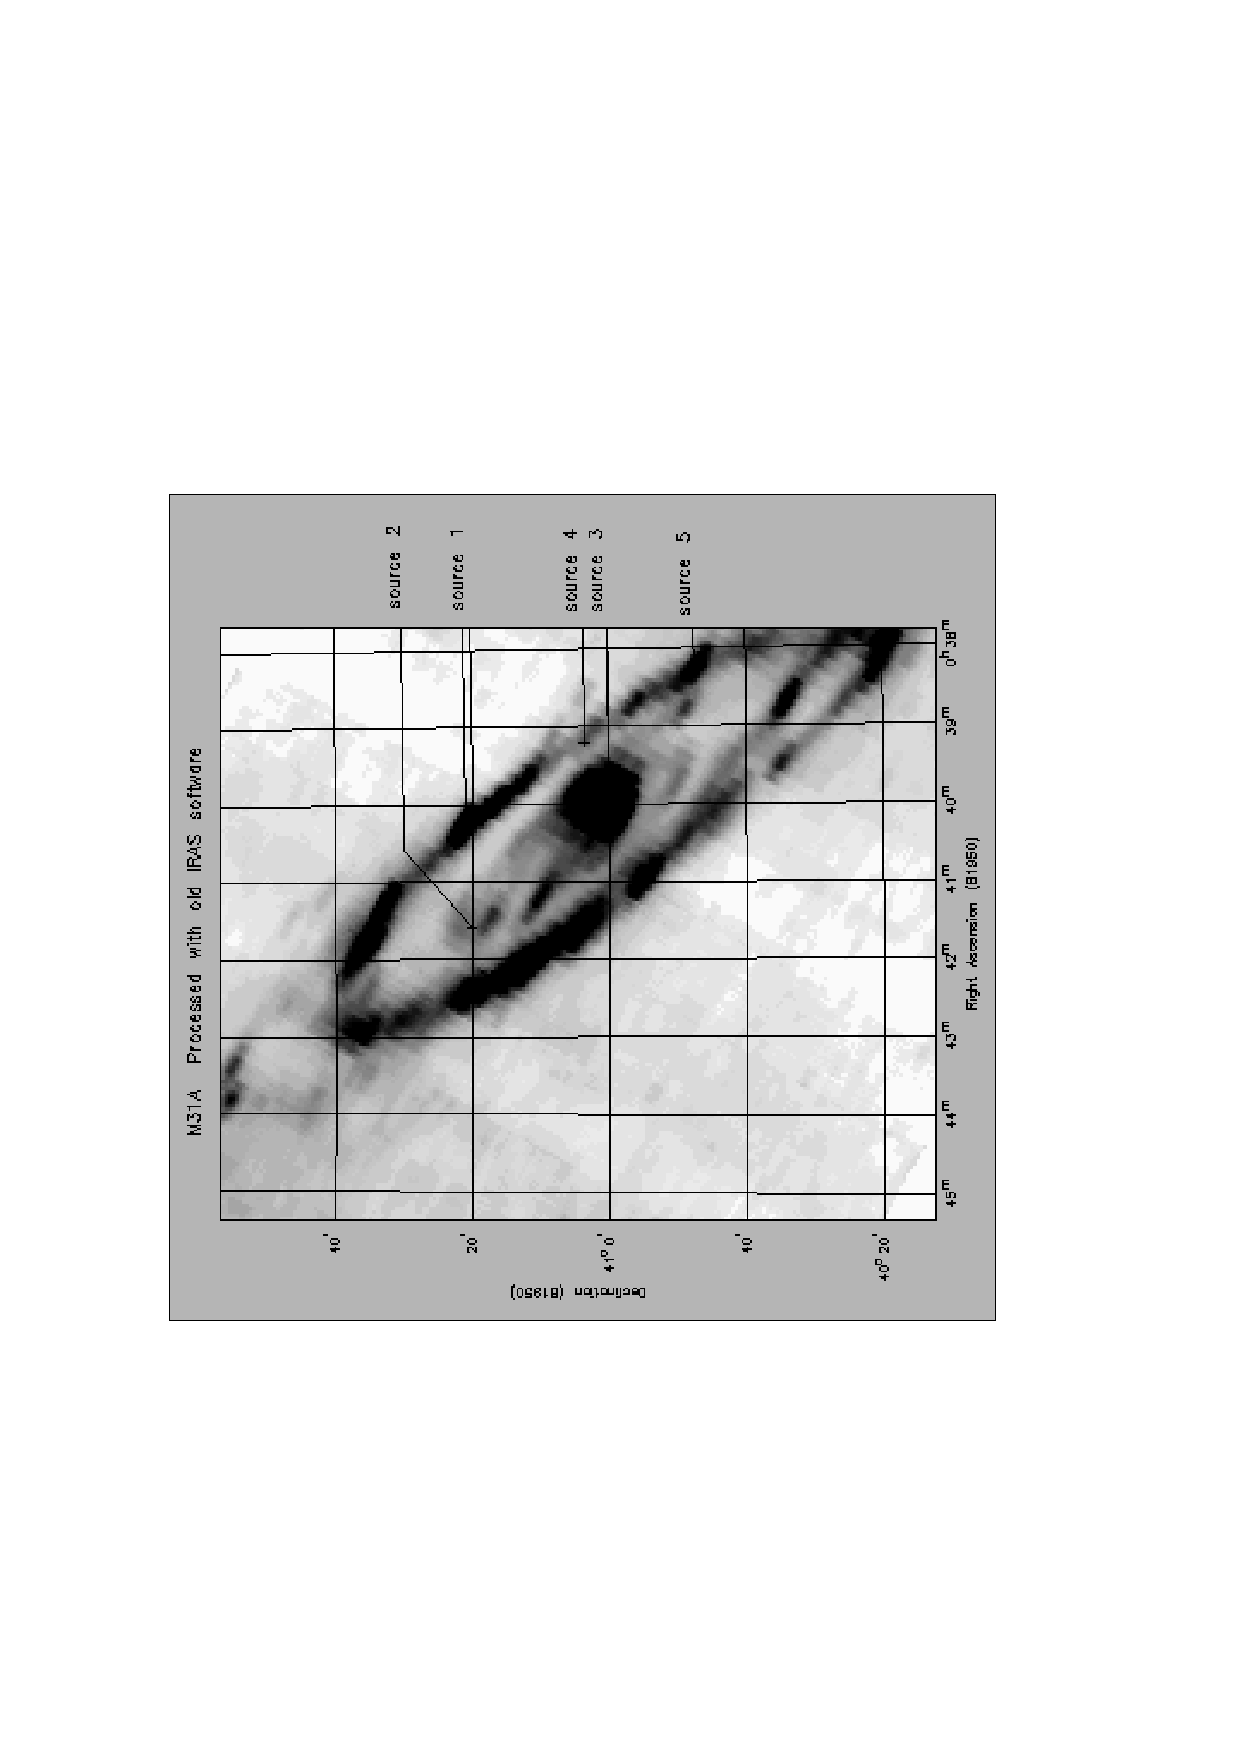
\includegraphics[width=\textwidth]{sun161_a_2_1}
\caption[KAPPA output of image]{KAPPA output of an image prepared with the old IRAS software
compared with that prepared with IRAS90}
\label{a:a2}
\end{figure}

\begin{figure}[h]
Figure not available. Only in Canon format.
\caption{I\_CONTOUR  output of old IRAS software image}
\label{a:a3}
\end{figure}

\begin{figure}[h]
\begin{tabular}{cc}
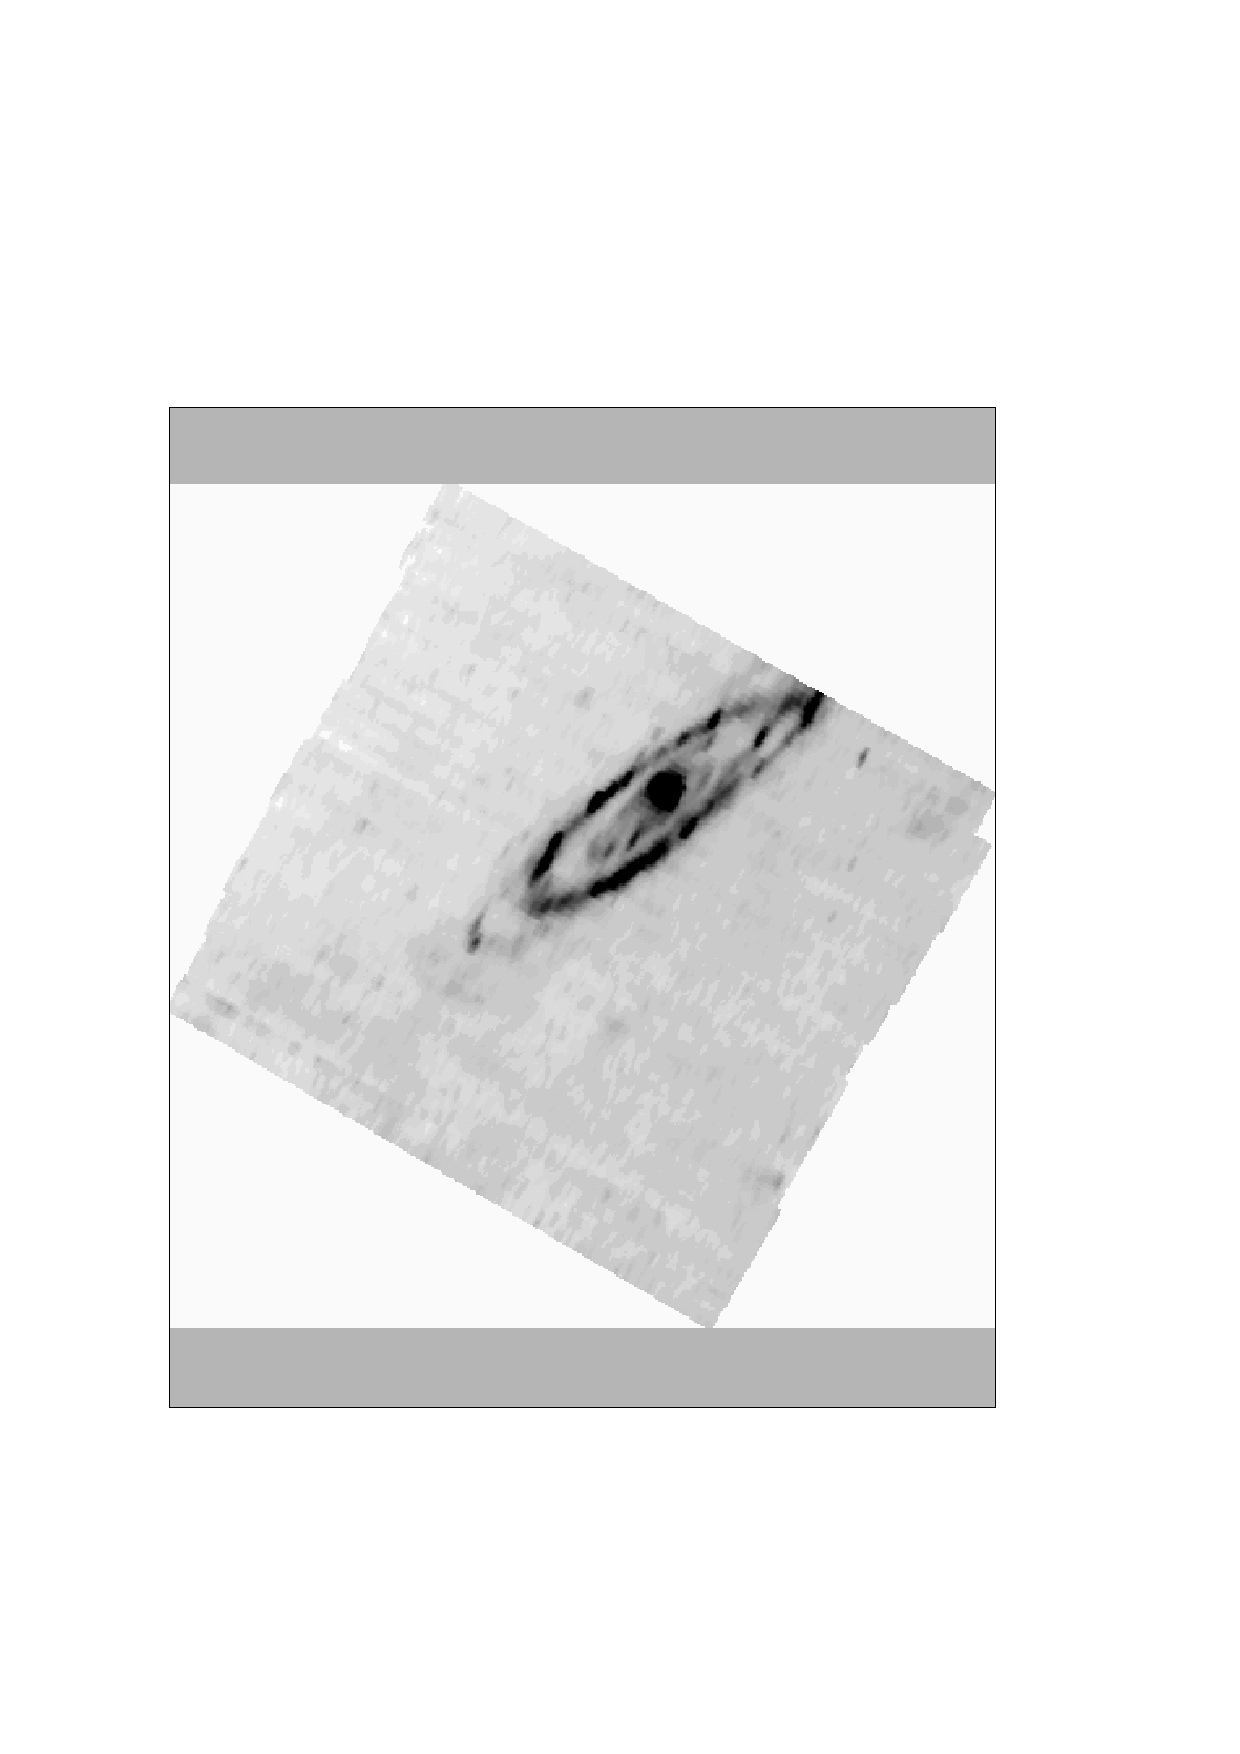
\includegraphics[width=0.4\textwidth]{sun161_a_4_1} &
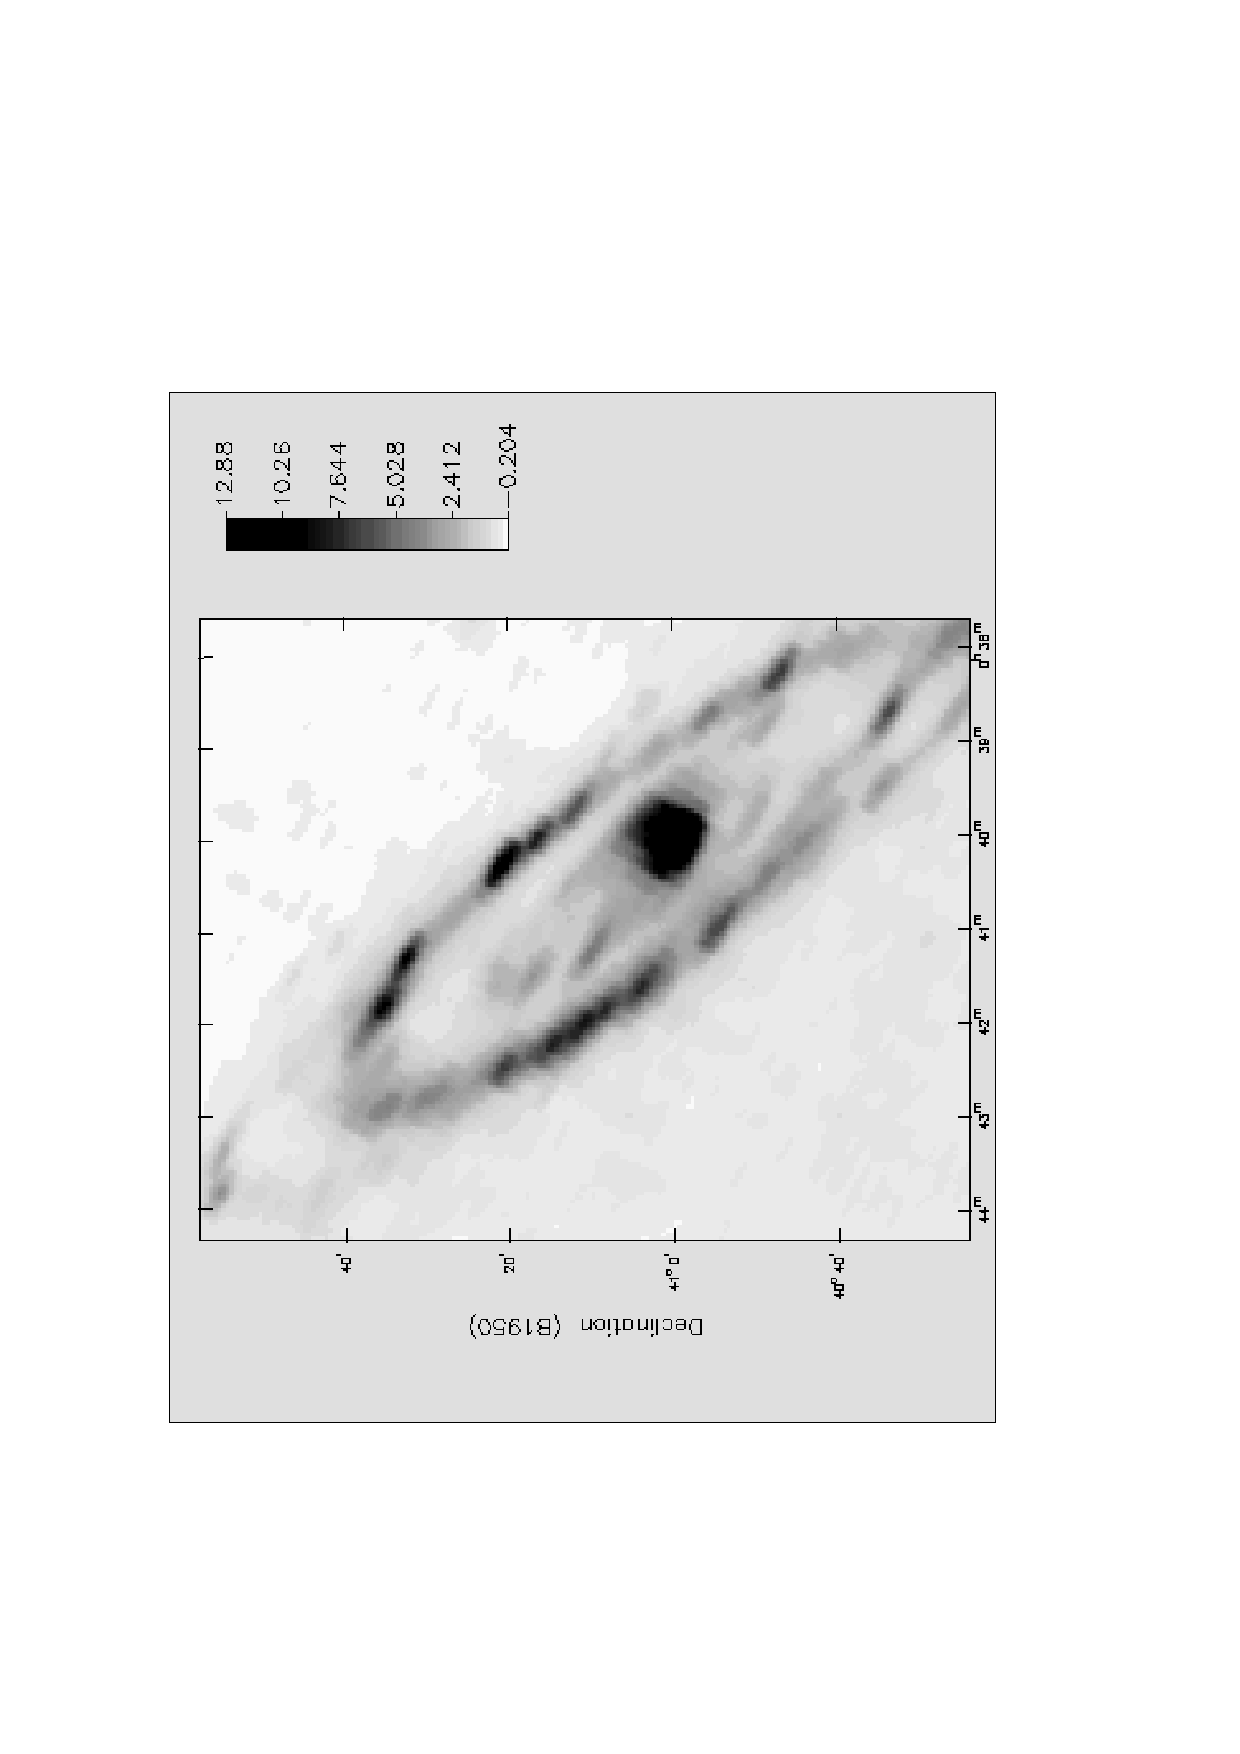
\includegraphics[width=0.4\textwidth]{sun161_a_4_2} \\
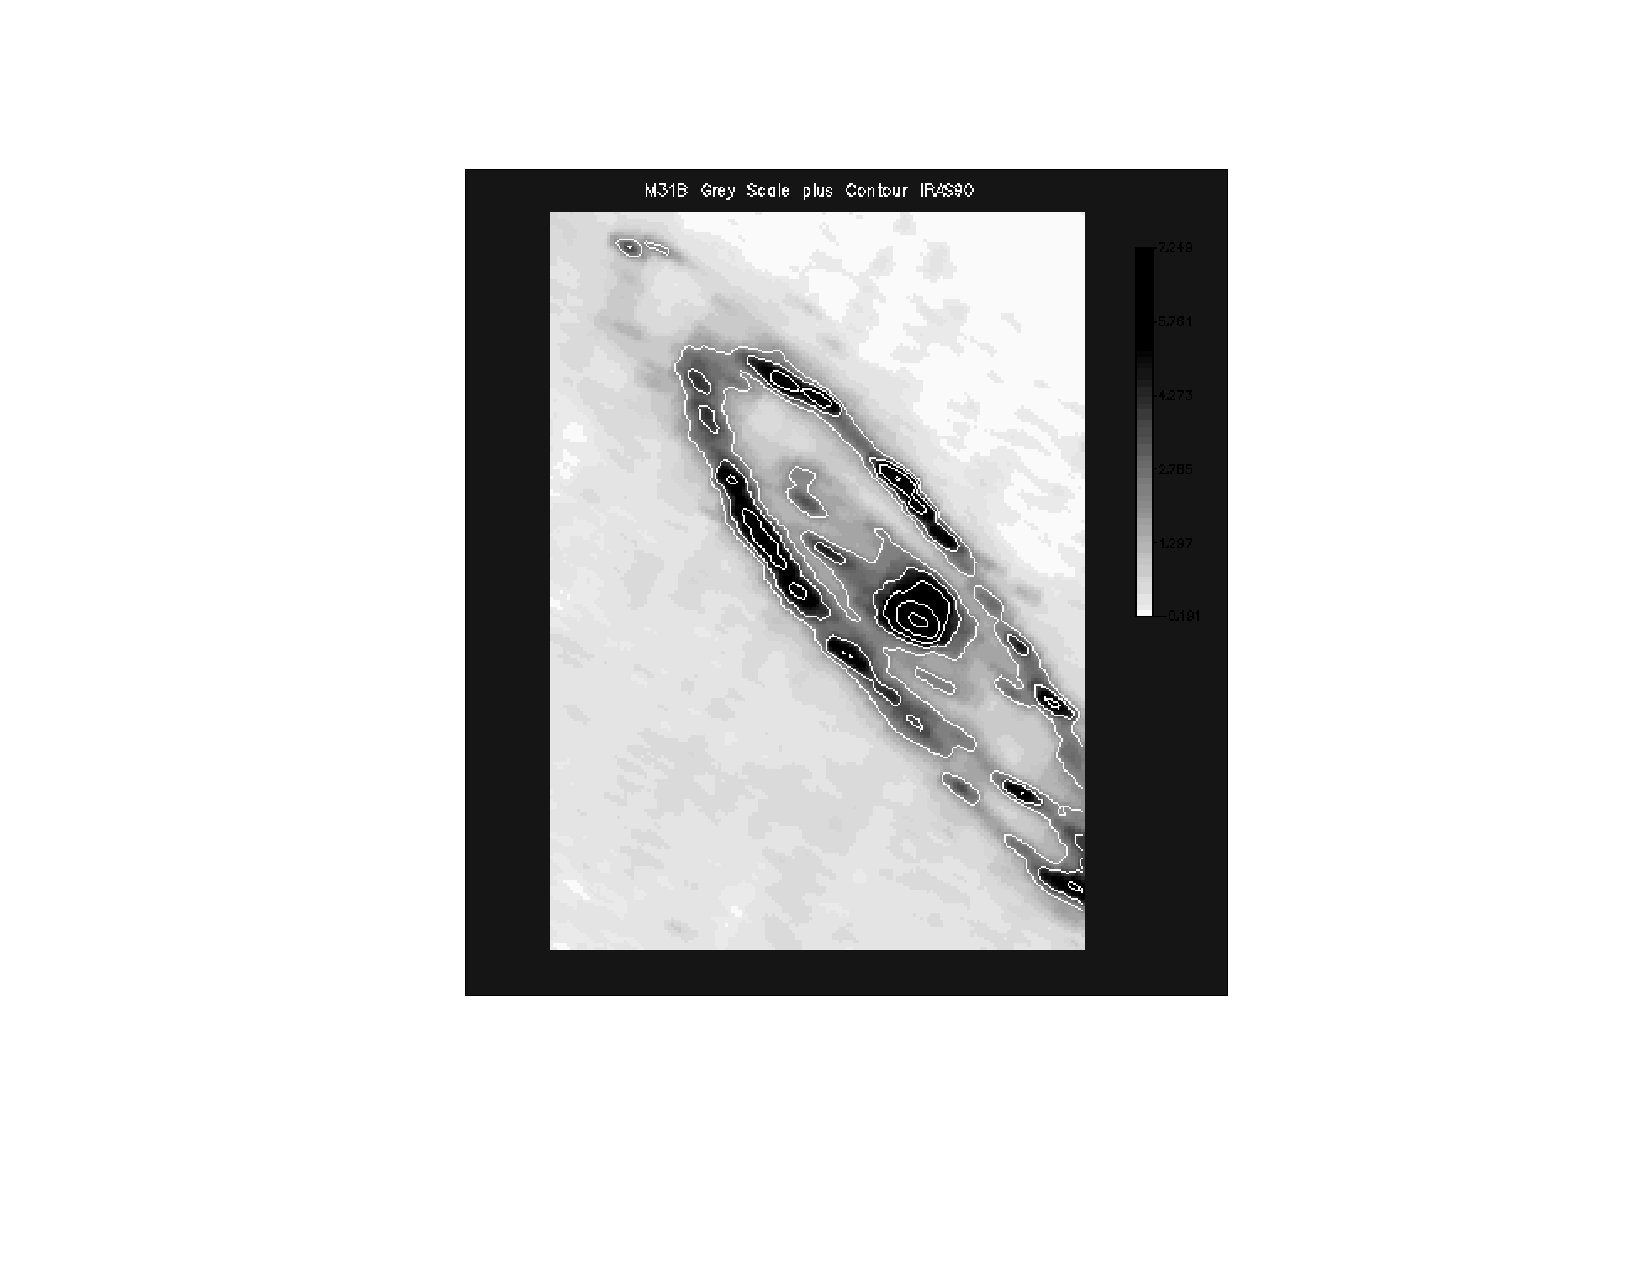
\includegraphics[width=0.4\textwidth]{sun161_a_4_3} &
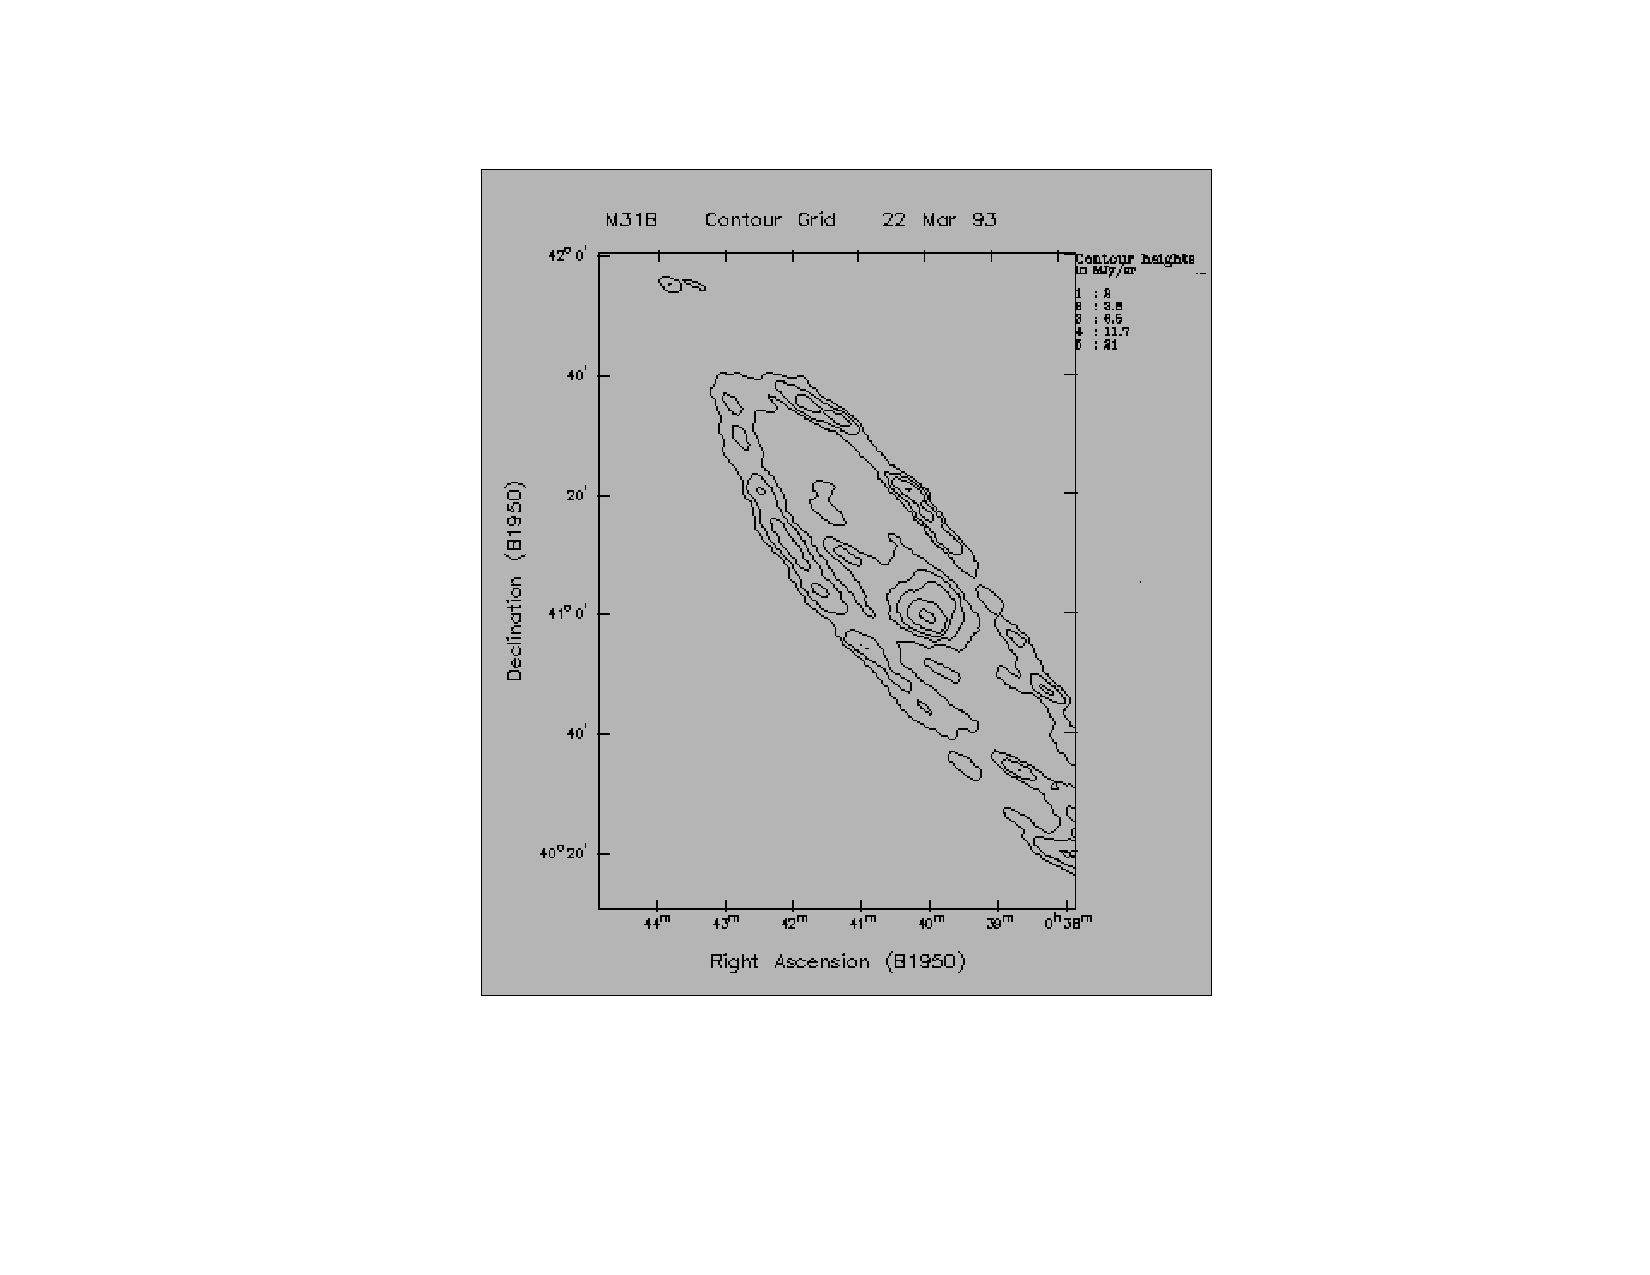
\includegraphics[width=0.4\textwidth]{sun161_a_4_4} \\
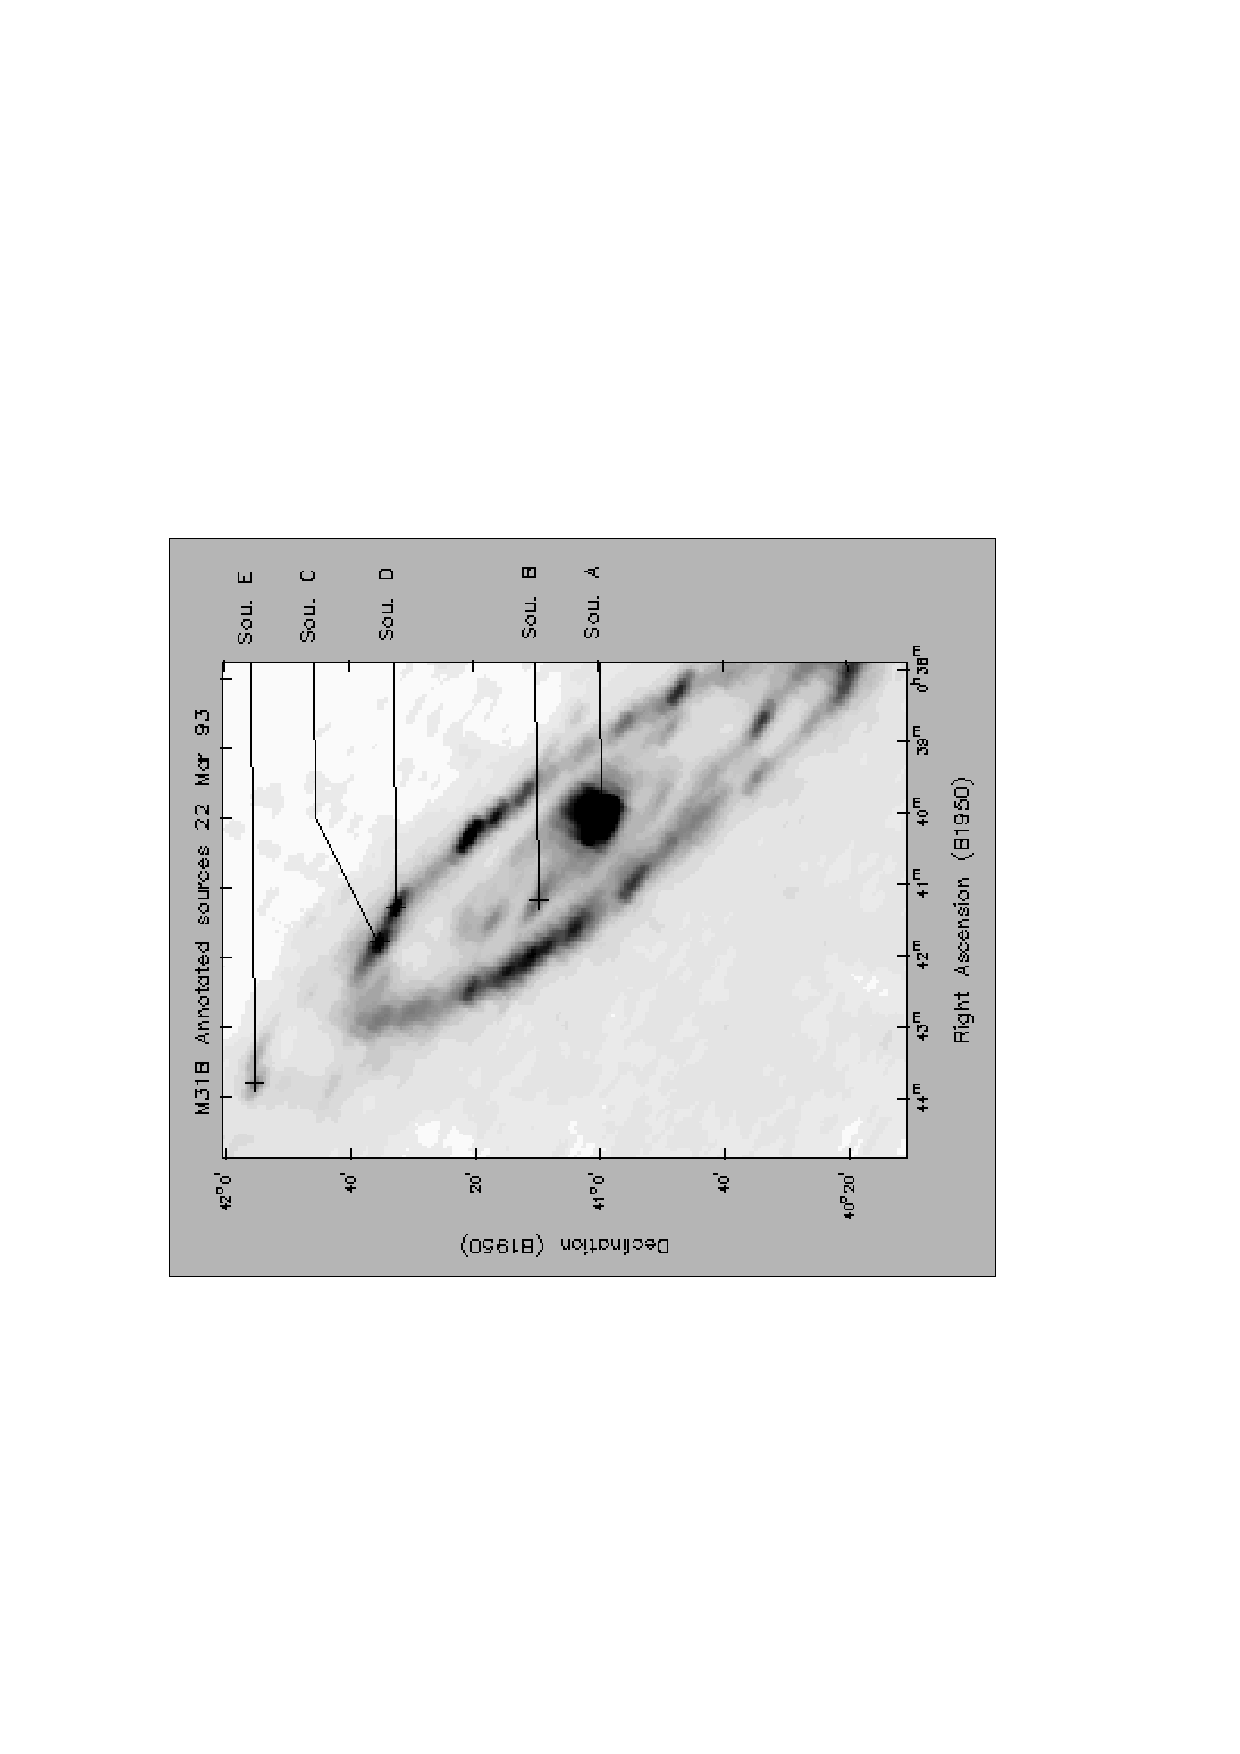
\includegraphics[width=0.4\textwidth]{sun161_a_4_5} & \\
\end{tabular}
\caption[Collection of KAPPA output images]{KAPPA output of  full image, subsection of image with grid, grey
scale image with contour map, gridded contour map, and grey scale image with
source positions.}
\label{a:a4}
\end{figure}

\clearpage

\section{Full prompts for DESTCRDD, BACKCRDD, \& MAPCRDD
\xlabel{full_prompts}\label{a:fulldbm}}

In this section full prompts for DESTCRDD, BACKCRDD and MAPCRDD are displayed.
The meanings of all the parameters are described in the relevant sections of
the IRAS90 documentation described in Appendix \ref{a:docs}. But these give the
parameters in alphabetical order, it is sometimes easier to see how parameters
relate to each other by looking at how the prompts are grouped. It is for this
reason that the user is given this section.
\begin{small}
\begin{terminalv}
$ destcrdd prompt
MSG_FILTER - Level of information to be displayed on the screen /'NORMAL'/ >
QEXP - Quality expression specifying usable CRDD /'ANY'/ >
BOX - Size of the smoothing box given as a number of samples /10/ >
CLIP - Number of standard deviations at which to clip data /3/ >
NITER - Number of cleaning iterations to perform /2/ >
IN - Input CRDD files /@m31b_b3_dsbk_h2/ > m31b_b3s11
OUT - Output CRDD files > m31c_b3s11_ds

  Processing DISK$IRAS:[IRAS90.TESTDATA]M31B_B3S11...

HISTORY - True if HISTORY is to be added to the output CRDD files /FALSE/ >
BACKMEAN - A dummy value to be replaced by the value of parameter BACKMEAN /0/ >
BACKSIGMA - A dummy value to be replaced by the value of parameter BACKSIGMA /0/
>
  The background surface brightnesses in the output CRDD files
  are distributed with a mean of 11.06631 MJy/sr and a standard
  deviation of 0 MJy/sr

$ backcrdd prompt
MSG_FILTER - Level of information to be displayed on the screen /'NORMAL'/ >
QEXP - Quality expression specifying usable CRDD /'ANY'/ >
CLIP - Number of standard deviations at which to clip data /3/ >
OUTBACK - Final background surface brightness (in MJy/sr) /0/ >
OUTTYPE - Type of output NDF required; DATA or BACKGROUND /'DATA'/ >
TYPE - Type of background to use /'UNIFORM'/ >
IN - Input CRDD files /@DISK$IRAS:[IRAS90.TESTDATA]M31C_B3S11_DS/ >
OUT - Output CRDD files > m31c_b3s11_ds_bk

  Processing DISK$IRAS:[IRAS90.TESTDATA]M31C_B3S11_DS...
    Background surface brightness is 11.06631 MJy/sr

HISTORY - True if HISTORY is to be added to the output CRDD files /FALSE/ >

$ mapcrdd prompt
MSG_FILTER - Level of information to be displayed on the screen /'NORMAL'/ >
COORDS - Sky coordinate system /'EQUATORIAL(B1950)'/ >
ORIENT - Position angle of the second image axis (the "Y axis") /0/ >
PROJTYPE - The map projection to use /'GNOMONIC'/ >
GAUSSIAN - True if Gaussian weighting is to be used /YES/ >
UNITS - Units for the output image /'MJy/sr'/ >
IN - The input CRDD files
/@DISK$IRAS:[IRAS90.TESTDATA]M31C_B3S11_DS_BK/ > m31b*bk
EXCLUDE - A set of detectors to exclude from the map /'SMALL'/ >
INCLUDE - The set of detectors to include in the map
/@"DISK$USER1:[DCP.ADAM]MAPCRDD.SDF;1"MAPCRDD.ADAM_DYNDEF.INCLUDE/ >
PIXSIZE - Output pixel dimensions in arc-minutes /0.5,0.5/ >

  12 CRDD files being mapped.

CENTRE_LON - Right Ascension (B1950) of the image centre /'0h 42m 52.00s'/ >
CENTRE_LAT - Declination (B1950) of the image centre /'41d 25m 17.71s'/ >
BOXSIZE - Dimensions of output image in arc-minutes /236.3174,232.472/ >
OUT - The output NDF containing the mapped CRDD > m31c_b3_dsbk_h2
TITLE - Title for output map /' M31A'/ >
FWHM - Cross- and in- scan FWHMs of Gaussian weighting function (arc-minutes)
/4.75,1.51/ >
SECSIZE - Cross- and in- scan sizes of a "sector" in arc-miutes /0.25,0.25/ >
VAROUT - Type of output VARIANCE values required /'NONE'/ >
QEXP - Quality expression specifying usable CRDD /'ANY'/ >

  Processing
DISK$IRAS:[IRAS90.TESTDATA]M31B_B3S11_DS_BK...
        .             .             .
        .             .             .
        .             .             .
  Processing
DISK$IRAS:[IRAS90.TESTDATA]M31B_B3S22_DS_BK...

HISTORY - True if HISTORY is to be added to the output NDF /FALSE/ >
\end{terminalv}
\end{small}
\newpage

\section{More complex KAPPA example - annotated diagrams,
and flux determinations
\xlabel{more_complex_kappa_example}\label{a:exkappa}}

In this more complex example of the use of KAPPA we  are aiming to carry out
two tasks, to obtain a neatly annotated diagram of centroid positions and
determine the flux at those positions, and to determine flux values at given
coordinate positions. It also provides an opportunity to give the user more
details of the type of tasks he can perform with some of the SKYPACK
applications.

\subsection {Task 1  - To obtain centroid positions for flux determination and
map of sources}
\label{a:exkappa1}
In this section the aim is to determine the centroid positions of certain
features on an image, to produce a greyscale image with the centroid positions
marked and annotated, and finally to determine the flux values of the pixels
under the centroid positions.

The first stage, that of finding the centroid positions, is easily carried out
using KAPPA's CENTROID.

It is assumed that the image from which the user wishes to obtain centroids is
already displayed, at a suitable scale, or with a suitable PICDEF. CENTROID is
run and the user positions the cursor at the approximate positions of
the center of each desired sub-region. CENTROID will provide the correct
positions of the centroids, and in the example below, will log these to the
`coout' file.
\begin{small}
\begin{terminalv}
$ centroid coout=m31b_centroid.log
Current picture has name: DATA, comment: KAPPA_DISPLAY.
Using DISK$IRAS:[IRAS90.TESTDATA]M31B_B3_DSBK_H2 as the input NDF.

Type a 1 or a space to select a point.
Type . to exit.
Use the cursor to select one point.

Input guess position was     63.463317871094, -48.471626281738
Output centroid position is  64.936340332031, -50.698829650879

Use the cursor to select one point.
           .                      .                 .
           .                      .                 .
           .                      .                 .
Use the cursor to select one point.
\end{terminalv}
\end{small}

The image pixel positions obtained with centroid can now be used, first to
find their sky coordinate positions for annotating the image, and secondly
for use with KAPPA's INSPECT to find the flux values.
\begin{small}
\begin{terminalv}
$ type/nopage m31b_centroid.log
64.936340332031  -50.698829650879
37.748733520508  -30.483295440674
24.218332290649  20.719131469727
35.053291320801  15.255108833313
-20.923727035522  60.530906677246
\end{terminalv}
\end{small}

The next section of the example is to provide the image with annotated source
positions. The annotation consists of three elements, the mark on the position,
the line to the edge of the image, and the text describing the source. To these
are finally added a grid and a title as in most of the other examples.
The source annotation takes place in the following stages.
\begin{itemize}
\item The centroid image positions are translated into sky positions, using
SKYPOS, and are then used to mark the position of the sources on the image,
using SKYMARK.
\item A trial run of SKYLINE in cursor mode is used to obtain approximate
positions for the lines from the marks to the edge of the image. These are
logged to a file. The file is the edited to give a file that can be input
to SKYLINE giving the required lines with a tidier spacing.
\item The overlay plane is cleared and the tidier lines are drawn using
SKYLINE and the file prepared in the last stage.
\item A trial run of SKYWRITE in cursor mode is used to obtain approximate
positions for the text strings at the end of the lines. These are logged to
a file, and the file is the edited to give the required text in a neater format.
\item The overlay plane is again cleared, and each of the marks, lines and text
are added using the corresponding application and file.
\item The grid and title are added using SKYGRID and SKYWRITE respectively, and
a file prepared for printing.
\end{itemize}

The first stage in developing the annotation is to mark the positions of the
sources using SKYMARK. To do this the user needs to edit the output file from
CENTROID to get a file of image coordinates which can be input into SKYPOS.
He can then run SKYPOS to translate the image coordinates into sky coordinates,
and log these sky coordinates to a file. He can use the file as input to SKYMARK
which will mark the positions on the image.

The output from CENTROID is the logfile listed above, this needs editing to give
the format below
\begin{small}
\begin{terminalv}
$ type m31b_centroid_mod.lis
IMAGE COORDINATE
#SOURCE A
64.936340332031
-50.698829650879
     .    .
     .    .
     .    .
#SOURCE E
-20.923727035522
60.530906677246
\end{terminalv}
\end{small}
The remainder of this stage can be carried out with the following instructions
\begin{small}
\begin{terminalv}
$ skypos mode=file file=m31b_centroid_mod.lis logfile=m31b_centr_mod_sky.lis

  Displaying EQUATORIAL(B1950) sky coordinates

IN - The NDF to which image coordinates refer /@M31B_B3_DSBK_H2(-44:114,-148:71)/ >

     RA                DEC                      X        Y

  0h 40m 0.03s,     40d 59m 48.75s    #  =     64.9    -50.7
  0h 41m 11.84s,    41d 10m 0.00s     #  =     37.7    -30.5
  0h 41m 47.28s,    41d 35m 37.57s    #  =     24.2     20.7
  0h 41m 18.20s,    41d 32m 54.33s    #  =     35.1     15.3
  0h 43m 48.18s,    41d 55m 31.81s    #  =    -20.9     60.5


$ t m31b_centr_mod_sky.lis
#  Log file from IRAS90:SKYPOS
EQUATORIAL(B1950)

#  Positions specified in file M31B_CENTROID_MOD.LIS
#    RA                DEC                      X        Y

  0h 40m 0.03s,     40d 59m 48.75s    #  =     64.9    -50.7
  0h 41m 11.84s,    41d 10m 0.00s     #  =     37.7    -30.5
  0h 41m 47.28s,    41d 35m 37.57s    #  =     24.2     20.7
  0h 41m 18.20s,    41d 32m 54.33s    #  =     35.1     15.3
  0h 43m 48.18s,    41d 55m 31.81s    #  =    -20.9     60.5

$ skymark mode=file file=m31b_centr_mod_sky.lis

  DATA picture "KAPPA_DISPLAY" being used
\end{terminalv}
\end{small}

The second stage is to carry out a trial run of SKYLINE to obtain approximate
positions for the lines, and to edit the resultant file.

\begin{small}
\begin{terminalv}
$ skyline loop

  DATA picture "KAPPA_DISPLAY" being used
  Using astrometry information stored in
  DISK$IRAS:[IRAS90.TESTDATA]M31B_B3_DSBK_H2
TYPE - Type of curve to draw /'poly'/ >

  Position the cursor at a vertex of the poly-line and press any button
(position the cursor outside the image to exit).
         .           .            .
         .           .            .
         .           .            .
TYPE - Type of curve to draw /'poly'/ > !
OPTION - Next operation /'CONTINUE'/ > save
LOGFILE - Output text file' /@M31B_SKYLINE_OUT.22MAR93/ >
OPTION - Next operation /'CONTINUE'/ > exit
$ t M31B_SKYLINE_OUT.22MAR93
# Curves drawn by SKYLINE over image

EQUATORIAL(B1950)  # Sky Coordinate System

Polyline
  0h 40m 6.84s, 41d 0m 39.00s
  0h 38m 57.95s, 41d 8m 50.96s
  0h 37m 50.95s, 41d 8m 41.27s

Polyline
  0h 41m 11.36s, 41d 33m 26.81s
  0h 37m 44.35s, 41d 34m 30.03s
  0h 32m 59.22s, 41d 34m 46.58s
\end{terminalv}
\end{small}
\begin{itemize}
\item The ! response to the TYPE prompt indicates that the user has finished
drawing lines and now wants to go on to the next option, which is to save the
specification of the lines drawn to the logfile.
\end{itemize}

The output from SKYLINE is compared with the sky coordinates of the centroid
positions output by SKYPOS. A suitable file is prepared giving two vertices
for each polyline for all sources except source C. These two vertices are the
source position and a position at the same Declination but with an RA taking
the line to the edge of the image. The line for source C looks as if it will
become confused with that for source D, so a three vertex polyline is specified
for this source giving a bend in the line. The edited SKYLINE file looks as
follows.
\begin{small}
\begin{terminalv}
$ t m31b_skyline_input.lis
EQUATORIAL(B1950)   #Sky Coordinate System

#SOURCE A SKYPOSITION_ M31A
#X = 64.93634,  Y = -50.69883
POLYLINE
0h 39m 59.93s       #LONGITUDE SOURCE
40d 59m 48.78s      #LATITUDE  SOURCE
0h 37m 00.00s       #LONGITUDE EDGE
40d 59m 48.78s      #LATITUDE EDGE

#SOURCE B
       .         .        .
       .         .        .

#SOURCE C
#X = 24.21833,  Y = 20.71913
POLYLINE
0h 41m 47.23s       #LONGITUDE SOURCE
41d 35m 38.15s      #LATITUDE SOURCE
0h 40m 00.00s       #LONGITUDE INTERMEDIATE
41d 45m 38.15s      #LATITUDE INTERMEDIATE
0h 37m 00.00s       #LONGITUDE EDGE
41d 45m 38.15s      #LATITUDE EDGE

#SOURCE D
       .         .        .
       .         .        .

#SOURCE E
#X = -20.92373,  Y = 60.5309
POLYLINE
0h 43m 48.24s       #LONGITUDE SOURCE
41d 55m 32.73s      #LATITUDE SOURCE
0h 37m 00.00s       #LONGITUDE EDGE
41d 55m 32.73s      #LATITUDE EDGE
\end{terminalv}
\end{small}
For the next stage the tidier lines are redrawn and a trial run of SKYWRITE in
cursor mode is used to obtain approximate positions for the text strings at the
end of the lines.
\begin{small}
\begin{terminalv}
$ ovclear
$ skyline mode=file file=m31b_skyline_input.lis

  DATA picture "KAPPA_DISPLAY" being used
  Using astrometry information stored with the picture in the AGI database

$ skywrite loop

  DATA picture "KAPPA_DISPLAY" being used
  Using astrometry information stored with the picture in the AGI database

  Position the cursor at a text position and press any button (position the
cursor well outside the image to exit).

TEXT - Text to be written > Sou. A
OPTION - Next operation /'CONTINUE'/ > at
ATTRIBUTE - Text attribute to set /'DEFAULT'/ > JUSTIFICATION
JUST - Text justification /'BC'/ > BL
ATTRIBUTE - Text attribute to set /'DEFAULT'/ > !
OPTION - Next operation /'CONTINUE'/ >

  Position the cursor at a text position and press any button (position the
cursor well outside the image to exit).
TEXT - Text to be written > Sou. B
OPTION - Next operation /'CONTINUE'/ > save
LOGFILE - Output text file' /@M31B_SKYWRITE_OUT.LIS/ >
OPTION - Next operation /'CONTINUE'/ > exit
$ t M31B_SKYWRITE_OUT.LIS
# Strings written by SKYWRITE over image

EQUATORIAL(B1950)     # Sky Coordinate System
DEFAULT

0h 37m 39.75s,41d 34m 29.26s, "Sou. A"

JUSTIFICATION, BL

0h 37m 40.29s,41d 8m 39.50s, "Sou. B"
\end{terminalv}
\end{small}
\begin{itemize}
\item The first prompt for the OPTION parameter was used to change the
justification of the text relative to the cursor position so that the cursor
was positioned at the bottom left of the text string.
\item The ! response to the ATTRIBUTE prompt indicates that no more attributes
are to be changed.
\item The save response to the third OPTION prompt indicates that the user has
finished adding text and now wants to go on to the next option, which is to save
the specification of the text to the logfile.
\end{itemize}
The output from SKYWRITE is compared with the sky coordinates of the last
vertex for polyline for each source, specified in the SKYLINE file. A suitable
file is prepared giving the text position for each source at the same
Declination as the end of its line, but with an RA which starts the text
slightly to the right of the image. The RA is the same for each source. The
amount of text that can be written is limited, about 7  characters for any
string. The final edited file is shown below.

\begin{small}
\begin{terminalv}
$ t M31B_SKYWRITE_INPUT.LIS
# Strings written by SKYWRITE over image

EQUATORIAL(B1950)     # Sky Coordinate System
DEFAULT
JUSTIFICATION, BL
# Source A
0h 37m 30.00s, 40d 59m 48.78s, "Sou. A"
# Source B
0h 37m 30.00s, 41d 10m 0.50s, "Sou. B"
# Source C
0h 37m 30.00s, 41d 45m 38.15s, "Sou. C"
# Source D
0h 37m 30.00s, 41d 32m 52.99s, "Sou. D"
# Source E
0h 37m 30.00s, 41d 55m 32.73s, "Sou. E"
\end{terminalv}
\end{small}
Finally the overlay plane is cleared again and the final annotated image is
redrawn.
\begin{small}
\begin{terminalv}
$ ovclear
$ skyline mode=file file=m31b_skyline_input.lis

  DATA picture "KAPPA_DISPLAY" being used
  Using astrometry information stored with the picture in the AGI database
$ skywrite mode=file file=M31B_SKYWRITE_INPUT.LIS

  DATA picture "KAPPA_DISPLAY" being used
  Using astrometry information stored with the picture in the AGI database
$ skymark mode=file file=m31b_centr_mod_sky.lis

  DATA picture "KAPPA_DISPLAY" being used
$ skygrid

  DATA picture "KAPPA_DISPLAY" being used
  The picture covers the image section ( -44:114, -148:71 )
  Using astrometry information stored with the picture in the AGI database

$ skywrite

  DATA picture "KAPPA_DISPLAY" being used
  Using astrometry information stored with the picture in the AGI database

  Position the cursor at a text position and press any button (position the
cursor well outside the image to exit).
TEXT - Text to be written > M31B Annotated sources 22 Mar 93
\end{terminalv}
\end{small}

To find flux values at centroid coordinates we must be careful to round the
centroid positions to the correct pixel number. The image positions should be
rounded \emph{up} as follows
\begin{small}
\begin{terminalv}
   Original Centroid            Correct
   Image Position              Pixel Value
   64.936340332031                 65
  -50.698829650879                -50
   37.748733520508                 38
  -30.483295440674                -30
   24.218332290649                 25
   20.719131469727                 21
                    etc.
\end{terminalv}
\end{small}

We now inspect the values at those coordinate positions.
\begin{small}
\begin{terminalv}
$ inspect mode=interface
IN - Image to be inspected /@M31B_B3_DSBK_H2(-44:114,-148:71)/ >
GDEVICE - Graphics device to be used for line plots /@x2w/ >
OPTION - Option required /'REGION'/ > value
VAIND - Pixel indices /[35,-38]/ > 65,-50

   VALUE of image at 65, -50 is 25.09315

OPTION - Option required /'VALUE'/ >
        .          .            .
        .          .            .
        .          .            .
OPTION - Option required /'VALUE'/ > ex
\end{terminalv}
\end{small}
\subsection {Task 2  - To determine flux values at given coordinate positions.}
\label{a:exkappa2}
The user should first use SKYPOS to translate the sky coordinate positions he
wants to examine to image coordinate values, in this example they are to be
logged to a file.
\begin{small}
\begin{terminalv}
$ skypos inverse mode=keyboard logfile=m31b_sky_to_image_coord.lis

  Displaying EQUATORIAL(B1950) sky coordinates
IN - The NDF to which image coordinates refer /@M31B_B3_DSBK_H2(-44:114,-148:71)/ >
LON - Right Ascension (B1950) of the required position > 0h 39m 59.93s
LAT - Declination (B1950) of the required position > 40d 59m 48.78s

      X         Y              RA               DEC

     64.9   , -50.7   #  =  0h 39m 59.93s    40d 59m 48.78s
               .                 .                .
               .                 .                .
               .                 .                .
               .                 .                .
LON - Right Ascension (B1950) of the required position > !

$ t m31b_sky_to_image_coord.lis
#  Log file from IRAS90:SKYPOS
IMAGE COORDINATES

#  Positions specified using the keyboard
#     X         Y              RA               DEC

     64.9   , -50.7   #  =  0h 39m 59.93s    40d 59m 48.78s
       .        .                .                 .
       .        .                .                 .
       .        .                .                 .
    -20.9   ,  60.5   #  =  0h 43m 48.24s    41d 55m 32.73s

\end{terminalv}
\end{small}

The flux values at the corresponding image coordinate can now be found, as
described in finding values for centroid positions above. Again care should be
taken in rounding the image coordinate values before using INSPECT to
determine the flux values.

\section{Quality
\xlabel{quality}\label{a:quality}}

The IRAS90 suite allows the user to set up `qualities' associated with data
pixels or samples, and to process data while including only data with
certain qualities in the calculations.  For example the user may wish to set
flags against certain detector samples marking them either `Source A' or
`Saturated' and then DESTRIPE the scan data file while excluding both `Source A'
and `Saturated' samples from the calculations of the destriping constants, yet
still obtaining final scan values in which the constants have been applied to
all samples.
\subsection{Assigning qualities to samples or pixels}
To ascribe a quality to a set of samples or pixels the user has merely to
specify an unused quality name and nominate the samples or pixels that are to
have that quality. There is a limit to how many quality names can be valid for
a  given scan file, or image file, but this is around eight names. Hidden from
the user a flag bit is set up for each name, for each sample or pixel. This
means that a sample or pixel can have any combination of all the valid
qualities.

There are two programs which can set samples, or pixels to have a quality.
\begin{itemize}
\item TRACECRDD provides the user with a means of defining selected samples to
have a new or a preexisting quality. To do this the user must first make sure he
is looking at the scan region and detectors to which he wants to assign this
quality. He then selects `Assign Quality' at the NEXT prompt. He is given a
cursor controlled box whose corners he then moves to cover the region and the
detector or detectors to which he wants to ascribe the desired quality. When he
has selected the box he will be asked to nominate the quality name, \emph{e.g.}
 SourceA.
He may either nominate a preexisting quality or a new one.
\item SETQUAL allows the user to specify quality on either a CRDD file or an
image file. The user has two options,
\begin{itemize}
\item He can list those samples, or pixels, he wishes to be given a specified
quality, by specifying their scan or image coordinates.
\item He can specify the samples or pixels to be assigned a quality by
supplying a mask file in which the corresponding pixels or samples are given a
`bad' value. This is of particular use for images where
\begin{itemize}
\item The KAPPA application SETMAGIC can be used to set all pixels of a given
value to the `bad' value.
\item The KAPPA application THRESH can create mask images where values above or
below threshold values can be set to the `bad' value.
\item The KAPPA application ZAPLIN can create mask images where rectangular
boxes can be set to the `bad' value.
\end{itemize}
\end{itemize}
SETQUAL has various options which allow the user to specify, for example, all
the pixels specified should be given the quality, or all the pixels other than
those specified should not have the quality.
\end{itemize}
\subsection{Carrying out calculations using quality }
In many IRAS90 applications, including DESTCRDD, BACKCRDD and MAPCRDD,
calculations can be carried out, or images formed, using only those samples
which fulfill a quality criterion. Thus specifying
\begin{small}
\begin{terminalv}
$destcrdd IN=M31A_B3S12 QEXP=.NOT.(SOURCEA.OR.SATURATED)
\end{terminalv}
\end{small}
will cause scan M31A\_B3S12 to have its destriping constants calculated omitting
any sample which is either Source A or Saturated or both.

The value given to QEXP is termed a quality expression. A quality expression
consists of either
\begin{itemize}
\item A single valid quality name, or
\item A correctly formulated Boolean expression consisting of
\begin{itemize}
\item Valid quality names
\item .NOT.,
\item .AND.,
\item .OR.  - (inclusive or),
\item .XOR. - (exclusive or),
\item .EQV. - ( equivalent, either both TRUE or both FALSE),
\item The constants .TRUE. and .FALSE.
\item Any parentheses needed to ensure the correct order of operation. (The
natural precedence of these operators is in the order given above)
\end{itemize}
\end{itemize}
\subsection{Displaying quality}
The user may want to display quality in two types of contexts, either quality
associated with scans, or quality associated with images. In each case a
pictorial mode of inspection is available.
\begin{itemize}
\item For users wanting to view quality associated with scans, TRACECRDD offers
him the option of viewing only those samples which meet a quality expression
criterion. The user should select Quality Expression at the PARAM prompt, and
enter a suitable quality expression to the QEXP prompt. The program will then
draw only those sections of the detector scans which meet the quality
expression.
\item A user wanting to look at quality associated with an image cannot view it
directly with KAPPA. He has to prepare an intermediate image in which all the
pixels fulfilling a quality expression are set to `bad' values, and
then view the resulting image with KAPPA. The program QUALTOBAD prepares such an
intermediate image. This can be simple setting of pixels of a specified quality
to bad, or a more complex specification which can provide more flexibility. Thus
if a user wanted to see only a single source region in an image containing
several, he would
\begin{itemize}
\item Prepare a THRESHOLDed image in which all the pixels above a source cutoff
value had been set `bad'.
\item Prepare a ZAPLINed image in which a rectangular box covering the source
region he wants to view had been set `bad'.
\item Use SETQUAL to set up two qualities on the original image, THRESH and
ZAPPED, each using one of the images prepared above as a mask to set pixels
corresponding to those with bad values to have the appropriate quality.
\item Prepare an intermediate image in which all pixels except those in the
single source region are set `bad'  by using
\begin{small}
\begin{terminalv}
$qualtobad IN=M31B_B3_H1 OUT=M31B_B3_H1_SA QEXP=.NOT.(THRESH.AND.ZAPPED)
\end{terminalv}
\end{small}
\item He can now DISPLAY the image with KAPPA, or use INSPECT to add all the
flux values in the image.
\end{itemize}
\end{itemize}
\subsection{Propagating quality}
DESTCRDD and BACKCRDD propagate quality settings from their input scans to the
output ones. However MAPCRDD which prepares images from scans does not propagate
quality as there is no well defined relationship between input samples and
output  pixels.
\subsection{Quality housekeeping routines}
\begin{itemize}
\item SHOWQUAL shows the quality names associated with the input file, or files.
\item REMQUAL removes quality names and the corresponding sample or pixel
settings, this enables a user to remove unwanted qualities so that he can set
up new ones.
\end{itemize}
\newpage

\section{When to use new format .SDF files, when to use old .BDF format, and
how to translate them
\xlabel{when_to_use_new_format_sdf_files}\label{a:ndfout}}

All the new IRAS90 applications, and KAPPA use new format .SDF files. Only
if the user wants to COADD point source data, for which he must use I\_COADD
at present will he need old format .BDF files. He should specify for what he is
going to use the data when he requests it. If the user wants to use both
I\-COADD and TRACECRDD on data he will need it in both formats, or he can
translate .BDF data to .SDF format.

The program NDFOUT can be used to change old format .BDF files to new format
.SDF files. This is particularly useful in translating scan files between
formats although in the example given below it is an image file that is being
translated. This program is not available under Unix as yet. The user can either
set up a logical name to the directory containing EDRSX, or run the program from
EDRSX as shown in the two examples below. Using a logical name it should be run
as follows
\begin{small}
\begin{terminalv}
$runstar ndfout_dir:ndfout

--> Give value for parameter INPUT
The input BDF image or CRDD file

INPUT:=m31a_b3_h2

Incarnations of the input exist with the following data types:
Signed longword (specify as "SL")
Real            (specify as "real")

--> Give value for parameter DTYPE

The interim data type of the input incarnation to use. This is only
prompted for if more than one incarnation exists in the input BDF

DTYPE /SL/ := <ret>

--> Give value for parameter BAND

The IRAS band number of the data contained within an input image.
The legal values are 1,2,3 or 4 corresponding to the 12,25,60 and 100 nm wavelength

BAND:= 3

--> Give value for parameter OUTPUT

The name of the output NDF. The format of the NDF ( SIMPLE or
PRIMATIVE ) is defined by the parameter NDFFORM

OUTPUT /m31a_b3_h2/:= <ret>

Output NDF contains 76295 bad data values
\end{terminalv}
\end{small}

If the user is running the program under EDRSX then he should access the program
by typing
\begin{small}
\begin{terminalv}
$ DSCL

DSCL> GO EDRSX

EDRSX> ndfout
\end{terminalv}
\end{small}

The prompts from there forward should be the same.

There are two programs that are useful to examine resultant NDF files.
IRASTRACE reads and checks the .NDF file and identifies whether it is a valid
IRAS image or scan format. Running TRACE enables  the user to look at the
contents of the sections of the .NDF file, the extensions in particular. Details
of TRACE can be found in \xref{SUN/102}{sun102}{}.

\section{Further documentation
\xlabel{further_documentation}\label{a:docs}}

\subsection{IRAS Documentation}
\subsubsection {General documentation on IRAS}
\begin{itemize}
\item \textbf{\xref{SUN/82}{sun82}{}} - `IRAS90 -- Data Products Primer'
\item \emph{IRAS Catalogs and Atlases: Explanatory Supplement}, 1988. ed. C.A.
Beichman, G. Neugebauer, H.J. Habing, P.E. Clegg, and T.J. Chester (Washington,
DC:GPO) --- This will be found in the libraries of most institutes.
\end{itemize}
\subsubsection {Documentation on previous IRAS CRDD processing}
\begin{itemize}
\item \textbf{\xref{SUN/91}{sun91}{}} - `IRAS -- Calibrated Raw Detector Data
Analysis User Guide'
\end{itemize}
\subsubsection {Introductory documentation on IRAS90}
\begin{itemize}
\item This document.
\item \textbf{\xref{SUN/80}{sun80}{}} - `IRAS90 -- Extraction and Preparation
of IRAS Images - User Guide'
\end{itemize}
\subsubsection {Higher level user documentation on IRAS90}
\begin{itemize}
\item \textbf{\xref{SUN/163}{sun163}{}} - `IRAS90 -- IRAS Survey and PO Data
Analysis Package - Reference Guide'
\end{itemize}
\subsection{Non IRAS Documentation}
\subsubsection{ADAM Users Documentation}
\begin{itemize}
\item \textbf{\xref{SG/4}{sg4}{}} - `ADAM -- The Starlink Software Environment'
\item \textbf{\xref{SUN/95}{sun95}{}} - `KAPPA -- Kernel Application
Package' - Introductory section.
\end{itemize}
\subsubsection{KAPPA and associated program users documentation}
\begin{itemize}
\item \textbf{\xref{SUN/95}{sun95}{}} - `KAPPA -- Kernel Application Package'
\end{itemize}
\subsection{Utility programs both IRAS and other}
\begin{itemize}
\item \textbf{SUN/24} - `ASPIC -- Image Processing Programs (2)' contains such
details as there are about NDFOUT in the EDRSX section
\item \textbf{\xref{SUN/55}{sun55}{}} - `CONVERT -- A Format-conversion Package'
contains details of BDF2NDF.
\item \textbf{\xref{SUN/102}{sun102}{}} - `TRACE -- Listing HDS Data Files'
\item \textbf{\xref{SUN/130}{sun130}{}} - `GWM -- X Graphics Window Manager'
\end{itemize}

\subsection{Programmers Documentation}
\begin{itemize}
\item Note that all programs are self documenting in that they have been
liberally prologued and commented.
\end{itemize}
\subsubsection{Documentation on utility routines}
Documents on the utility routines, IRA, IRC etc, are held as IDxx.TEX files
in the .DOC subdirectory of the IRAS90 release version.
\end {document}
